
\documentclass[masters,nocolorlinks]{seuthesix}
\usepackage{style}

\begin{document}
\categorynumber{TU312} % 分类采用《中国图书资料分类法》
\UDC{624}            %《国际十进分类法UDC》的类号
\secretlevel{公开}   % 学位论文密级分为"公开"、"内部"、"秘密"和"机密"四种
\studentid{140926}   % 学号要完整,前面的零不能省略
\title{大跨越输电塔结构在龙卷风作用下的响应分析}{}{Response analysis of long span transmission tower structure under tornado wind loading}{}
\author{王勇}{Yong WANG}
\advisor{吕令毅}{教授}{Ling-yi LYU}{Prof.}
\degreetype{工学硕士}{Master of Engineering} % 详细学位名称
\major{土木工程}
\submajor{结构工程}
\defenddate{2017-06-01}
\authorizedate{}
\committeechair{史治宇}
\reviewer{S005127-1}{S005127-2}
\department{东南大学土木工程学院}{School of Civil Engineering}
\seuthesisthanks{}

\makebigcover
\makecover

\begin{abstract}{龙卷风数值模拟;大跨越输电塔结构;静力弹塑性分析;参数化分析;动力时程分析}
  % 摘要写法
  %% 第一段:研究对象介绍;研究意义;目前研究不足之处;本文主要研究问题
  %% 第二段-第四段:
  %%% 本章主要研究问题;
  %%% 采用的研究方法;
  %%% 主要结果。
  龙卷风是一种伴随着高速旋转的漏斗状云柱的强风涡旋,发生的概率较低,但破坏力巨大。
  大跨越输电塔结构是重要的生命线电力工程设施,具有数量大、分布广等特点,容易造成龙卷风的袭击,其破坏将导致供电系统的瘫痪甚至引发火灾等严重后果,造成重大经济损失。
  美国输电塔设计规范已考虑龙卷风等极端天气荷载,我国相关设计规范尚未涉及。 为保障龙卷风多发地区电网运行安全,进行输电线路的龙卷风荷载及抗风研究具有重要的理论和实用价值。
  本文利用计算流体动力学(CFD)模拟技术和规范方法,研究龙卷风数值风场的生成和其作用于大跨越输电塔结构的静态荷载和考虑龙卷风移动效应的动态荷载,分析典型工况下输电塔结构的响应。
  
  首先,研究利用CFD模拟技术建立龙卷风数值风场的方法。
  根据龙卷风的试验模拟文献,并参考前人的数值模拟方法,建立了相应于缩尺龙卷风发生装置的CFD数值模型。
  模拟结果表明数值风场的切向速度的分布与Rankine涡模型及试验测量的风速分布吻合较好,验证了缩尺龙卷风数值风场的可靠性。
  并将缩尺龙卷风数值风场与1998年发生在Spencer地区的龙卷风实测风场进行对比,通过长度相似比和速度相似比的概念将缩尺风场模型改造成足尺模型。
  发现当长度相似比取为$4000$、速度相似比取为$60$时,龙卷风足尺数值风场与实测风场的切向速度分布吻合较好。
  
  其次,利用单向流固耦合(FSI)方法和规范方法计算龙卷风作用于输电塔结构的荷载,并分析比较结构响应。
  FSI方法直接在足尺龙卷风风场中建立输电塔结构的刚性模型,通过CFD方法计算得到结构表面受到的龙卷风风压,并将其转化为输电塔梁单元模型的节点集中力;
  规范方法利用输电塔设计规范中风荷载计算公式将足尺龙卷风数值风场转化为风荷载。
  然后在龙卷风典型袭击角度(\SI{0}{\degree}、\SI{45}{\degree}和\SI{90}{\degree})工况下,以两种方法计算输电塔结构受到的龙卷风荷载,进行静力弹塑性分析并分析结构响应。
  结果表明,采用FSI 方法计算得到的输电塔结构响应整体上小于规范方法,且最大轴向力误差不超过$20\%$,位移响应不超过$30\%$;
  两种方法计算的结构响应随龙卷风袭击角度的变化趋势相似,可实现两种龙卷风荷载计算方法的相互验证。
  
  最后,进行了输电塔结构在考虑龙卷风平移效应时的动态响应分析。
  选取龙卷风移动路径平行和垂直于输电线的两种典型工况,在任意时间步利用规范方法计算并施加龙卷风动态荷载,进行动力时程分析,并分析龙卷风动态荷载和结构典型响应的时程。
  结果表明,平行工况下龙卷风荷载总和时程在输电线方向的分量出现持续时间约为\SI{10}{s}的波形(荷载先逐渐增大,后逐渐衰减),且荷载峰值较大,呈现出一定的冲击效应。
  垂直工况下龙卷风荷载总和时程在垂直输电线方向的分量出现类似的特点。
  且在两种工况下,输电塔塔顶节点位移时程与龙卷风荷载总和时程变化趋势相似。

\end{abstract}

\begin{englishabstract}{}

\end{englishabstract}

%%% Local Variables:
%%% mode: latex
%%% TeX-PDF-mode: t
%%% TeX-engine: xetex
%%% End:


\tableofcontents

\mainmatter

\graphicspath{{figures/intro/}}

\chapter{绪论}

\section{课题研究背景及意义}
2016 年 6 月 23 日,江苏盐城发生一场 EF4 级龙卷风,对盐城市阜宁县、射阳县一带造成严重影响。
据当局统计,龙卷风至少造成 99 死,846 人伤,其中近 200 人重伤。
此龙卷风造成的伤亡是几十年来最严重的\cite{wiki2016yancheng}。
这一严重龙卷风灾引起了社会对极端天气现象的关注。

龙卷风是一种伴随着高速旋转的漏斗状云柱的强风涡旋,中心附近风速可达 \SI{100}{m/s} -- \SI{200}{m/s},甚至 \SI{300}{m/s}。

美国国家海洋和大气管理局对美国历年记录的龙卷风发生次数和等级的统计如图\ref{fig:tornado-years}所示\cite{noaa2017tornado}:
美国每年平均记录到 $1,200$ 次龙卷风,2000年后龙卷风发生次数各年间波动较大,产生这一波动的原因还未有定论。
这意味着以后可能会出现某些年份龙卷风出现次数非常多、而其余年份次数较少的情况。

\begin{figure}[!htbp]
    \centering
    \includegraphics[width=\textwidth]{toryears.png}
    \caption{美国龙卷风年发生次数统计}
    \label{fig:tornado-years}
\end{figure}

相比于美国,中国龙卷风发生的概率相对较小,平均每年不足 100 个,大多集中在中、东部地区,如长江三角洲、苏北、鲁西南、豫东平原等。
我国龙卷风发生的数量虽然不及美国,但其造成的损失也是巨大的,据统计我国平均每年有$17$个省(区、市)遭受龙卷风,每年因龙卷风造成的死亡人数都在$10$人以上,受伤人数超千人,受灾人数更是少则上万多则百万,造成的直接经济损失高达数十亿元\cite{liu2007chinese}。

尽管龙卷风每年对我国造成的损失是巨大的,但由于其发生的概率和影响范围相对较小,目前我国《建筑结构荷载规范》中尚未包含普通建筑结构的抗龙卷风设计要求,但对一些重大工程如核电常规岛,一旦遭受破坏,其后果将不堪设想,我国已明确要求此类工程必须考虑结构的抗龙卷风设计。

大跨越输电塔结构是重要的生命线电力工程设施,具有数量大、分布广等特点,容易遭受龙卷风的袭击,其破坏将导致供电系统的瘫痪甚至引发火灾等严重后果,造成重大经济损失。

2016 年江苏盐城龙卷风中,共计 220 座各类通信基站退服,倒杆 2800 根,部分地区出现影响电力供应中断和通信基站无信号的情况,1570 根有线信号杆线受损,162 杆路灯损坏,40 条高压供电线路受损,影响 3 万负荷供电;
射阳县电力、通讯杆线受损严重,龙卷风经过的 4 条 10 千伏线路区域用户全停。
在当地的阿特斯协鑫阳光电力科技有限公司的两座厂房损毁,损毁面积达 4 万平方米\cite{thepaper2016yancheng}。
输电线路的破坏直接影响了救援救伤的效率,造成了灾区人民生命财产的重大损失。

2003 年 4 月 12 日,广东河源遭受罕见的龙卷风袭击,输电系统遭到重创,205 座高压输电线杆塔、440 条线杆被折断或者刮倒\cite{zhang2006shudianxian}。

据统计,全球范围内约$80\%$的输电塔倒塌破坏是由于极端天气(如龙卷风、雷暴等)的影响\cite{hamada2010finite}。
这主要因为大跨越输电塔结构具有塔体结构高、跨距大、柔性强等特点,是风敏感性结构,这就需要在其设计中考虑龙卷风荷载。
美国输电塔设计规范已考虑龙卷风等极端天气荷载,但我国输电线路设计规范尚未涉及。
鉴于近年龙卷风发生频率和强度似有增大趋势,而以往国内针对输电塔受龙卷风袭击的研究较少。
故为保障龙卷风多发地区电网运行安全,进行输电线路的龙卷风荷载及抗风研究具有重要的理论和实用价值。

\section{龙卷风荷载研究现状}
龙卷风是强对流天气的产物,是一种小尺度的高速旋转的气旋,具有突发性、区域性、短暂性、强破坏性,其风场特性不同于常规风。
迄今为止,人们对于龙卷风的发生机理尚未彻底清楚,但学者从未停止对龙卷风的研究。
从早期气象上的理论和实测研究,到如今的试验和数值模拟研究,获得了可供工程设计参考的相关数据。
这一过程中,龙卷风风场结构及其荷载的研究方法在不断地发展进步。
目前,国内外对龙卷风荷载的研究主要有现场实测、理论分析、试验模拟和数值模拟等方法,下文逐一介绍。

\subsection{现场实测研究}
现场实测是研究龙卷风最直直接且重要的方法。
但由于龙卷风发生地点及移动路径的随机性,研究者无法事先在其移动路径上安置观测仪器。
另外,龙卷风破坏力巨大,风场中常夹杂着飞射物,观测仪器容易遭受破坏丧失数据采集能力。
另一种现场实测方法是采用可移动的 Doppler 雷达来追踪并测量龙卷风。
但由于测量设备的限制,无法获得近地面风场的准确数据,而近地面数据又是工程抗龙卷风设计的重要参考数据,
这限制了现场实测数据在实际工程抗龙卷风设计中的应用。

即便如此,现场实测仍然为龙卷风风场结构、演化规律等的研究提供的宝贵数据。
爱荷华州立大学利用一种非常坚固的探测仪器,并在其内部设置朝向八个方向的摄像头,以便能从不同角度拍摄龙卷风内部情况。
根据拍摄的录像可以看到,龙卷风袭击低矮房屋时,房屋各个部分的破坏顺序为:首先是屋顶坍塌,然后是周围墙壁,最后是整个房屋倒塌。
房屋首先受到底部巨大风速的冲击,接着被旋风从外围袭击,最后被向上的气流摧毁。
Alexander(2005)\cite{alexander200530}利用移动的 Doppler 雷达获得了 1998 年 5 月 30 日发生于美国南达科他州的强龙卷风不同高度处的风速。
Kuai(2008)\cite{kuai2008cfd}等人对其数据进行处理,得到该龙卷风切向和径向风速分布分别如图\ref{fig:vt}和\ref{fig:vr}所示。
\begin{figure}[!htbp]
    \centering
    \includegraphics[width=0.6\textwidth]{spencer-vt.jpg}
    \caption{龙卷风切向风速沿径向的分布曲线}
    \label{fig:vt}
\end{figure}

\begin{figure}[!htbp]
    \centering
    \includegraphics[width=0.6\textwidth]{spencer-vr.jpg}
    \caption{龙卷风径向速度沿高度的分布曲线}
    \label{fig:vr}
\end{figure}

图\ref{fig:vt}为所测得的 \SI{20}{m} 到 \SI{660}{m} 高度处龙卷风的切向风速曲线。
龙卷风的切向风速曲线存在一个峰值,其核心半径随高度从\SI{120}{m}变化到\SI{250}{m},表现为漏斗形状。
图\ref{fig:vr}为龙卷风在不同径向位置处,径向风速随高度的变化曲线。
负值表示空气流入龙卷风内部,在离龙卷风中心\SI{1000}{m}处,\SI{400}{m}以下均为入流层。
但随着距离龙卷风中心距离越来越近,入流层的厚度逐渐减小。
最大径向速度出现在地面以上\SI{20}{m}高度处,这是雷达所能测得最低位置处的风速值。

目前龙卷风野外实测最大的研究项目是 VORTEX2 实验。
它是由美国科学基金会(NSF)和美国海洋和大气局(NOAA)共同组建,耗资 10 亿美元,
共有 100 多位研究者参与其中,出动雷达车共 10 部,启用近 40 个移动地面气象站,风暴边缘利用直升飞机探测。
该项研究的现场实测部分从 2009 年 5 月 1 日开始,于 2010 年 6 月 15 日结束。
所观测的范围从美国德克萨斯州的西部直到明尼苏达州的西南部,长达 1448 公里。

该项研究主要为了解决以下几个简单却很难回答的基本问题:
龙卷风是什么时候怎样形成的,为什么有些强烈并持续时间长而有些微弱且持续时间短;
龙卷风的结构是怎样的,它们靠近地面的风速有多大,是怎样对周围造成破坏的;
怎样可以更好地预报龙卷风,目前能提前预报龙卷风的时间平均为 13 分钟,
并且有 $70\%$的错误率,怎样可以更准确地预报,并且增加提前预报的时间。
初步数据显示 VORTEX2 一共捕获大约 30 个较大级别的龙卷风,
20 个强度较弱或寿命较短的龙卷风,其中有些龙卷风超过了 EF2 级。
所采集的龙卷风数据已在整理分析当中,但所测龙卷风原始数据的讨论和发表工作要在现场实测完成后的 5至7年内才能完成。

\subsection{试验模拟研究}
由于现场实测的困难和限制,研究者尝试建立缩尺龙卷风发生装置模拟龙卷风风场及其对结构的作用。
Chang \cite{chang1971tornado}在 1971 年最早使用实验装置模拟龙卷风,得到了内部风场的切向速度和径向速度,
发现这可作为有限的现场实测的补充,是一种有效的方法。
1972 年 Ward \cite{ward1972exploration}改进了 Chang 的龙卷风模拟装置,
改进的装置能仅允许近地面空气进入,并设置了滤去气流竖向涡量的蜂窝板。
此后许多龙卷风发生装置均是基于这个装置的改进。
1977 年普渡大学的 Church \cite{church1977tornado}设计了新型龙卷风模拟装置,采用旋转金属网实现气流的旋转。
1993 年 Lund 和 Snow为普度大学第二代龙卷风模拟装置中使用了激光多普勒测速仪,发现模拟的龙卷风风场的竖向速度、径向速度和切向速度的分布符合 Rankine 涡的特征。
该装置还采用了导流板代替了旋转的金属网,可以产生不同角度的入流速度。
2008 年 Mishra \cite{mishra2008physical}利用新的龙卷风模拟装置模拟出了速度场,并与 1998 年 5 月 30 日发生的曼彻斯特龙卷风和 2003 年 7 月 24 日发生在南达科他州的实测数据进行了对比,
发现二者的压力分布和切向速度分布吻合较好,这表明利用实验模型模拟龙卷风是可行的。
2008 年 Haan \cite{haan2009tornado}研究了不同龙卷风模拟装置设置对龙卷风涡结构及其大小的影响。

由于龙卷风发生装置可有效模拟龙卷风风场结构,研究者开始将不同类型的建筑物放置在发生装置中,用来研究龙卷风荷载。
1983 年 Jischke \cite{jischke1983laboratory}利用类似于 Ward 型龙卷风研究了圆柱形和长方体建筑物在龙卷风风场表面的风压分布,发现其与常规风洞实验的结果相差甚远,即建筑物表面受到的风压是在常规风场中的 3 至 5 倍,并指出龙卷风的最大风速、建筑模型的位置以及建筑模型与涡的相对方位是龙卷风造成破坏的重要因素。
2003 年爱荷华州立大学设计建成了可平行移动的龙卷风发生装置,内部可放置缩尺比 $1/150$ 到 $1/300$ 的结构模型。
2006 年,爱荷华州立大学的 Sarkar 和 Haan \cite{haan2009tornado}对 \SI{54}{m}宽,\SI{216}{m}高的缩尺比例为$1/500$ 的长方体房屋进行了研究,发现当龙卷风等级为 F2 级时,龙卷风荷载超过了美国土木工程师协会(ASCE7-02)规定的荷载值,约为美国沿海地区风荷载的 1.8 倍。
2008 年 Mishra \cite{mishra2008physical}利用德州理工大学的漩涡 2 号模拟装置(TTU-VSII)对不同径向位置处立方体建筑上的龙卷风作用进行了实验研究,给出了可渗透建筑(其内部的压力与龙卷风压相平衡)的表面压力系数。
研究表明,当建筑物位于所模拟龙卷风的边缘时,只有一个面为正压,这与大气边界层流中的情况比较类似。
随着建筑物不断靠近龙卷风中心,龙卷风的涡流影响越来越大。
2010 年 Haan \cite{haan2009tornado}等人利用爱荷华州立大学(ISU)的移动龙卷风模拟装置模拟人字屋顶建筑上的龙卷风荷载。
实验结果表明,建筑侧面风吸力的峰值是吹直风时的 $1.5$ 倍,竖向力系数峰值是一般规定的 $2$ 到 $3$ 倍,这可能是由于龙卷风中心存在较大负压的影响。
2012 年 Sabareesh 等人\cite{sabareesh2012dependence}通过东京理工大学的龙卷风模拟装置,研究了固定龙卷风中不同位置及地形环境中的建筑物表面风压分布情况。
当建筑物位于龙卷风核心半径处时,与切向流相垂直建筑表面的负压相对于其他表面较小。
2013 年 Rajasekharan \cite{rajasekharan2013characteristics}利用东京理工大学的龙卷风模拟装置,研究了建筑物在龙卷风中的位置以及两种不同开洞方式对建筑物内部压力、屋顶净风力的影响。

国内龙卷风方面的试验研究起步较晚,2013 年,东南大学的汤卓等建造了国内首个龙卷风发生装置,并将其命名为“龙卷风塔”,该试验装置如图\ref{fig:seu-tornado}和图\ref{fig:seu-tornado2}所示。
\begin{figure}[!htbp]
    \centering
    \includegraphics[width=0.6\textwidth]{tornado-sim.jpg}
    \caption{东南大学汤卓龙卷风发生装置}
    \label{fig:seu-tornado}
\end{figure}

\begin{figure}[!htbp]
    \centering
    \includegraphics[width=0.6\textwidth]{tornado-sim2.png}
    \caption{东南大学汤卓龙卷风发生装置原理图}
    \label{fig:seu-tornado2}
\end{figure}

利用此装置进行了龙卷风作用下双坡屋面风压分布的试验研究,结果表明:
龙卷风场的风速分布、风压分布以及总气压降和 Rankine 涡模型吻合较好,其试验结果也说明了龙卷风作用于建筑物的荷载与常规风作用存在较大差异。
2014 年,同济大学的王锦和周强等\cite{wang2014tornado}制造出了龙卷风试验装置。
该试验装置是基于 Haan 等的设计原理制作而成的,主要由顶部悬吊的控制风机、环状管道以及导流板组成。
该装置可以产生一定的平移速度,最大为 \SI{0.4}{m/s},试验过程中采用眼镜蛇探头测试龙卷风风场。
试验结果表明其模拟的切向速度和静压分布与真实龙卷风的监测结果较一致。

\subsection{数值模拟研究}
龙卷风的现场实测具有许多限制,难以准确观测近地面处(\SI{20}{m} 以下)的真实风场,
这限制了现场实测数据在实际工程抗龙卷风设计中的应用,因为近地面风场是工程设计主要关注的;
再者,龙卷风的解析模型(如 Rankine 模型)是经过简化的理想模型,还不能贴近真实风场;
最后,即使是试验方法也受到缩尺比的限制,难以模拟真实龙卷风尺寸。
研究者开始寻找新的研究龙卷风的方法。

龙卷风数值模拟方法的研究,主要是在龙卷风缩尺试验研究的基础上发展起来的。
1997 年,Lewellen 等人\cite{lewellen1997large}利用大涡模拟技术(Large Eddy Simulation, LES)模拟了一个单涡龙卷风结构,
并研究其与地面的相互作用,解释了形成龙卷风结构所需的条件,
还指出 Rankine 涡模型是满足 Navier-Stokes 方程的最简单模型。
1999 年 Nolan 和 Farrel \cite{nolan1999structure}利用轴对称不可压缩流的数值模型研究了龙卷风结构的动力特性和结构特性,
发现旋转流场的角动量和湍流粘度直接影响龙卷风的结构。
2003 年 Selvam 和 Millett \cite{selvam2003computer}利用 Rankine 涡模型给出了数值模拟龙卷风风场的速度边界条件,
并利用 LES 方法计算了立方体表面作用的龙卷风荷载,
发现平移的龙卷风模型产生比准定常模型更大的作用力,墙体要增加$45\%$,屋顶要增加将近一倍。
2008 年 Kuai 等人\cite{kuai2008cfd}以爱荷华州立大学的龙卷风模拟装置为基础进行了数值模拟,
表明数值模拟结果可较好吻合实验数据,若考虑地面粗糙度,数值模型可更好模拟雷达观测的数据。
2011 年 Nashimi 等人\cite{alrasheedi2011computing}利用 LES 方法对同一龙卷风尺寸,不同建筑物尺寸(建筑平面尺寸从一倍变到八倍,高度保持不变),
龙卷风和平行常规风分别作用于建筑物的荷载进行了对比研究,
发现随着建筑物平面尺寸的增大,龙卷风风场中建筑物的竖向阻力系数最多可减少$80\%$,
侧向阻力系数和轴向阻力系数最多可减少$90\%$。
2012 年 Natarajan 等人\cite{natarajan2012large}利用 LES 方法研究龙卷风平移速度及地面粗糙度对龙卷风风场的影响,
发现随着地面粗糙度的增加,减小了模拟龙卷风的最大切向速度,
而龙卷风平移速度对风场最大切向速度的影响不能得到统一结论,切向速度出现减小和略微增大两种不同情况。

国内针对龙卷风的数值模拟研究日趋增多。
2005 年同济大学的陈艾荣\cite{chen2004large}基于准定常理论对大跨斜拉桥在龙卷风作用下的响应做了分析研究,
发现了龙卷风对斜拉桥的竖向托起效应。
2009 年湖南大学的甘文举\cite{gan2009low}通过涡运动理论,建立了考虑龙卷风平移运动的数值风场模型,对低层房屋的龙卷风荷载及抗风设计提出了实用计算的建议。
2011 年,河北大学刘伟\cite{liu2011lou}采用了 Realizable 湍流模型模拟了龙卷风风场特性,并模拟了不同体型的建筑物位于风场中不同位置时的受力情况。
同年,哈尔滨工业大学李波利用 Fluent 对影响龙卷风风场的各种参数进行了分析,还得到了风场中建筑物表面和附近的速度与风压的分布特征。
2012 年,东南大学汤卓\cite{tang2012tornado}利用 CFD 数值模拟方法模拟了龙卷风作用于大跨穹顶结构的研究,获得了大跨穹顶结构表面的风压系数和作用在结构上的龙卷风荷载时程曲线,并对大跨穹顶结构作了风致响应分析。
2012 年,哈尔滨工业大学徐枫\cite{xu2013tornado}采用 Fluent 模拟了龙卷风风场特性,并对比理论模型从而验证了模拟结果的合理性。
2013 年,唐飞燕\cite{tang2013tornado}探讨了龙卷风风场中沙粒对结构冲击作用。
2014 年,东南大学王兆勇\cite{wang2015different}利用湍流模型模拟了在等效移动龙卷风作用下不同坡角的双坡屋面模型的风压分布特征,并与静态龙卷风风场特性相比,发现等效移动龙卷风风场中风压激增现象更加明显,双坡屋面风荷载急剧增大。

\section{本课题研究现状}
目前国外研究龙卷风作用下输电塔结构响应的文献较少。
Savory(2001)\cite{savory2001modelling}采用龙卷风 Wen 模型(忽略龙卷风风场竖向速度),利用风力系数将风速场转化为输电塔结构所受的风荷载,并考虑了龙卷风的平移运动,在其行进路径垂直于输电线的典型工况下进行动力时程分析,并根据输电塔结构的动态响应分析其破坏形态。
Langlois(2007)\cite{langlois2007design}主要评估了 ASCE、Behncke 等提出的多种龙卷风简化荷载模型对输电塔结构响应的影响。
其中的龙卷风简化荷载模型假定输电塔所受的风压是均匀分布的,并且忽略了风场的竖向分量及风场对输电线的作用。
Hamada(2010)\cite{hamada2010finite}利用缩尺 CFD 模型进行龙卷风风场的数值模拟,然后根据 ASCE No.74 规范提出的计算方法将 CFD 风场转化为输电塔结构受到的风荷载,然后进行静力弹塑性分析。
并改变龙卷风核心相对于输电塔结构的位置,分析其对输电塔结构响应的影响。
Hamada(2011)还进行了考虑龙卷风平移运动时输电塔结构动力时程分析,思路与 Savory 类似,只是将龙卷风场采用 CFD 模拟风场,进一步考虑了龙卷风平移路径与输电线平行的工况。
Altalmas(2014)\cite{altalmas2014finite}研究思路与 Hamada 类似,进行了更详尽的参数分析,即龙卷风核心相应于输电塔的角度、距离这两个参数对输电塔结构响应最值的影响。

任超(2010)\cite{ren2010tower}仅考虑了龙卷风的平移速度和最大切向速度,利用《架空送电线路杆塔结构设计技术规定》的风荷载计算公式将其转化为输电塔结构受到的龙卷风荷载,进行静力弹塑性分析。
白俊峰(2011)\cite{bai2011tornado}利用 Rankine 龙卷风涡模型计算出空间桁架表面对应的风压,进行龙卷风作用下输电塔结构的静力计算,发现与相同风速下自然风作用下的结构响应很相近。

由此可见国内外文献研究龙卷风作用下输电塔结构响应的基本思路为:采用 Rankine 或 Wen 模型模拟龙卷风解析风场,或采用 CFD 技术模拟龙卷风数值风场;
然后利用规范中风荷载计算公式将风速场转化为风荷载并施加到输电塔有限元模型上,计算结构响应。
这一研究思路采用自然风作用下的风荷载参数(如体型系数等)计算龙卷风荷载,但龙卷风与自然风风场结构相差较大,有必要研究直接模拟输电塔结构所受龙卷风荷载的方法。
另一方面,国外的研究成果难以直接用于国内的输电塔结构抗龙卷风设计的参考,主要原因在于国内外输电塔结构体系存在不同之处,所以需要选取中国典型的输电塔工程进行建模计算;
另一个原因在于国内外将风场转化为风荷载的计算公式不同,因此需要利用中国规范或标准的风荷载计算公式评估龙卷风的作用。

\section{本课题主要研究内容}
第二章:
建立龙卷风数值风场模型。
以 Baker 实验为基础,利用 Fluent 软件建立缩尺龙卷风风场模型,将 CFD 计算得到的数值龙卷风风场的风速分布与 Baker 实验进行对比,以验证模拟结果的正确性。
并将缩尺风场与实测 Spencer 龙卷风风场进行对比,引入足尺风场与缩尺风场的长度相似比和速度相似比,以探讨将缩尺龙卷风数值风场转化为足尺风场的方法。

第三章:
龙卷风作用下输电塔结构的静态响应分析。
利用单向流固耦合方法(下文简称 FSI)直接在足尺龙卷风风场中建立输电塔的刚性模型,进行 CFD 计算得到结构表面受到的龙卷风风压。
结构有限元计算采用梁单元模拟输电塔结构,故需研究将 CFD 计算得到的结构表面风压转化为梁单元节点集中力的方法。
本章还介绍了利用规范方法计算龙卷风荷载并施加到输电塔结构的方法。
最后改变龙卷风的袭击角度,分别在 0 度、45 度和 90 度工况下进行龙卷风荷载的计算和施加,
进行静态响应计算,并比较两种方法计算得到的结构轴向力和位移响应。

第四章:
龙卷风作用下输电结构的动态响应分析。
考虑龙卷风的平移运动,建立动态龙卷风风场及荷载模型。
针对龙卷风运动典型工况(移动路径平行于输电线、移动路径垂直于输电线),分析输电塔典型节点所受龙卷风风速及风载时程,进行动力时程分析,提取结构位移响应时程曲线。

%%% Local Variables:
%%% mode: latex
%%% TeX-PDF-mode: t
%%% TeX-engine: xetex
%%% End:

\graphicspath{{figures/tornado/}}
\chapter{龙卷风风场及其数值模拟}\label{chapter:tornado}

\section{引言}
龙卷风比常规风具有更为复杂的风场结构,且具有突发性、生存时间短、发生区域较小、破坏性较强等特点。
这些特点为龙卷风的研究带来了较大难度。
目前常用的研究方法中,现场实测受到测量仪器等因素的限制,难以获得近地面风场数据;
解析方法建立了简化的理想风场模型,还不够贴近真实风场;
试验模拟方法也存在着模型尺寸、测量精度等方面的限制。
相比于以上三种研究方法,数值模拟方法,如计算流体动力学模拟方法(Computational Fluid Dynamics, CFD),具有成本低、周期短、效率高等优点:
首先CFD方法不受结构尺度和构造的影响,能进行足尺龙卷风风场的模拟;
其次可以测试不同模拟参数对风场结构的影响,进而探讨结构在不同风载工况下的响应变化;
最后,CFD技术可利用丰富的后处理和可视化工具,提供现场实测和试验模拟方法不便测量的流场信息。
因此,近年来CFD模拟方法日益广泛地应用于龙卷风的研究当中。

本章基于CFD数值模拟技术,探讨了模拟龙卷风足尺风场的方法。
首先阐述了CFD方法的基本理论,并介绍了龙卷风的主要性质和参数。
然后利用CFD软件ANSYS Fluent模拟了文献中龙卷风试验模型生成的风场,并与1998年发生在Spencer地区的实测龙卷风进行对比,通过引入长度相似比和速度相似比的概念将缩尺龙卷风风场转化为足尺风场。

\section{计算流体动力学基本理论}
% \section{计算流体动力学基本理论}
计算流体动力学(Computational Fluid Dynamics, CFD)是通过数值方法在计算机中对流
体力学的控制方程(质量守恒方程、动量守恒方程、能量守恒方程)进行求解,从而可预测
流场的流动。
CFD技术的基本思路可归纳为:把时间域及空间域上连续的物理量(如压力场、速度场),
用一系列的有限离散点上变量值得集合来代替,通过一定的原则和方式建立关于离散点上场
变量之间关系的代数方程组,然后求解此代数方程组获得场变量的近似值。

CFD克服了传统的理论分析和试验研究的缺点,不受物理模型和试验模型限制,经济、高效、
灵活,能够给出较为完整的数据和图像。
尤其对特殊情况如试验无法模拟的时候,CFD将会发挥出独特的优势。

\subsection{控制方程}

流体的流动要受物理守恒定律的支配,包括质量守恒定律、动量守恒定律和能量守恒定律。
控制方程是这些守恒定律的数学描述。

\subsubsection{质量守恒方程}
质量守恒定律可表述为:单位时间内流体微元体中质量的增加量,等于同一时间间隔内流入
该微元体的净质量。
根据这一定律,可得到流体的质量守恒定律(连续方程):
\begin{equation}
  \label{eq:continuity}
  \frac{\partial \rho}{\partial t} + \mathrm{div} (\rho \bm{u}) = 0
\end{equation}
式中:$ \rho $为空气密度,$ t $是时间,$ \bm{u} $为空气的速度矢量,$ u $、$ v $、
$ w $是速度矢量$ \bm{u} $在$ x $、$ y $、$ z $三个方向上的分量,$ \mathrm{div}
(\bm{a}) = \frac{\partial a_x }{\partial x } + \frac{\partial a_y }{\partial y }
+ \frac{\partial a_z  }{\partial z } $为矢量$ \bm{a} $的散度。

\subsubsection{动量守恒方程}
动量守恒定律可以表述为:流体微元体中流体动量对时间的变化率等于外界作用在该微元体
上的各种力之和,该定律实际上是牛顿第二定律。
据此,可推导出$ x $、$ y $、$ z $ 三个方向的动量守恒方程:
\begin{equation}
  \label{eq:momentum}
  \begin{cases}
    \rho \frac{\mathrm{d} u }{\mathrm{t}} = -\frac{\partial p}{\partial x} +
    \frac{\partial \tau_{xx}}{\partial x} + \frac{\partial \tau_{yx}}{\partial y} +
    \frac{\partial \tau_{zx}}{\partial z} + F_x \\
    \rho \frac{\mathrm{d} v }{\mathrm{t}} = -\frac{\partial p}{\partial y} +
    \frac{\partial \tau_{xy}}{\partial y} + \frac{\partial \tau_{yy}}{\partial y} +
    \frac{\partial \tau_{zy}}{\partial z} + F_y \\
    \rho \frac{\mathrm{d} w }{\mathrm{t}} = -\frac{\partial p}{\partial z} +
    \frac{\partial \tau_{xz}}{\partial x} + \frac{\partial \tau_{yz}}{\partial y} +
    \frac{\partial \tau_{zz}}{\partial z} + F_z \\
  \end{cases}
\end{equation}
式中:$p$为流体微元体上的压力;$\tau_{xx}$、$\tau_{xy}$、$\tau_{xz}$分别为因粘性
作用而产生的作用在微元体表面上粘性应力的分量;$F_x$、$F_y$和$F_z$是微元体上的体
力分量,当微元体受到的体力只有重力,且$z$轴的方向竖直向上时,体力可以写成:
$F_x=0$,$F_y=0$,$F_z=-\rho g$。

下面对流体的粘性应力进行分析。当相邻两层流体发生相对滑移(即剪切变形)时,在与变
形相反方向上会产生粘性应力(切向应力),来阻止变形的发生。
流体这种抵抗变形的性质,称为粘性。
结构风工程中的研究对象主要为近地层的空气,一般可看成是牛顿粘性流体。
对于牛顿粘性流体,流体的粘性应力与其变形率成比例,各分量可写成如下形式:
\begin{equation}
  \label{eq:newton}
  \begin{cases}
    \tau_{xx}=2\mu \frac{\partial u}{\partial x} + \lambda \mathrm{div} \bm{u} \\
    \tau_{yy}=2\mu \frac{\partial v}{\partial y} + \lambda \mathrm{div} \bm{v} \\
    \tau_{zz}=2\mu \frac{\partial w}{\partial z} + \lambda \mathrm{div} \bm{w} \\
    \tau_{xy}=\tau_{yx}=\mu \left( \frac{\partial u}{\partial y} +
      \frac{\partial v}{\partial x} \right) \\
    \tau_{xz}=\tau_{zx}=\mu \left( \frac{\partial u}{\partial z} +
      \frac{\partial w}{\partial x} \right) \\
    \tau_{yz}=\tau_{zy}=\mu \left( \frac{\partial v}{\partial z} +
      \frac{\partial w}{\partial y} \right)
  \end{cases}
\end{equation}
式中,$\mu$是动力粘度,$\lambda$为第二粘度,一般可取$\lambda=-\frac{2}{3}\mu$。
将式\eqref{eq:newton}代入式\eqref{eq:momentum}中,可得到牛顿流体的动量方程,也就
是比较常见的Navier-Stokes方程:
\begin{equation}
  \label{eq:ns}
  \begin{cases}
    \frac{\partial (\rho u)}{\partial t} + \mathrm{div}(\rho u \bm{u}) =
    \mu  \bm{\mathrm{grad} }(u) - \frac{\partial p}{\partial x} + S_u \\
    \frac{\partial (\rho v)}{\partial t} + \mathrm{div}(\rho v \bm{u}) =
    \mu \bm{\mathrm{ grad} }(v) - \frac{\partial p}{\partial y} + S_v \\
    \frac{\partial (\rho w)}{\partial t} + \mathrm{div}(\rho w \bm{u}) =
    \mu \bm{\mathrm{ grad} }(w) - \frac{\partial p}{\partial x} + S_w
  \end{cases}
\end{equation}
式中,$\bm{\mathrm{grad}}() = \frac{\partial ()}{\partial x} \bm{i} + \frac{\partial
  ()}{\partial y} \bm{j} + \frac{\partial ()}{\partial z} \bm{k}$为变量的梯度;
$S_u$、$S_v$、$S_w$代表着动量守恒方程的广义源项,其中$S_u=F_x+s_x$,
$S_v=F_y+s_y$,$S_w=F_z+s_z$,一般情况下,$s_x$、$s_y$、$s_z$是小量,此处不再列
出,对于粘性为常数的不可压缩流体,可取$s_x=s_y=s_z=0$。

\subsubsection{能量守恒方程}
能量守恒定律是包含有热交换的流动系统必须满足的基本规律,能量守恒定律可表述为:流
体微元体中能量的增加率等于进入微元体的净热流量加上体力与面力对微元体所做的功。
该定律实际上是热力学第一定律。
\begin{equation}
  \label{eq:energy}
  \frac{\partial \rho T}{\partial t} + \mathrm{div} (\rho \bm{u} T) =
  \mathrm{div} \left( \frac{K}{c_P} \bm{\mathrm{grad}} T \right) + S_T
\end{equation}
式中:$T$是流体的温度,$K$是流体的传热系数,$c_p$是比热容,$S_T$是流体的内热源及
由于粘性作用流体机械能转换为热能的部分,有时简称$S_T$为粘性耗散项。

综合方程\eqref{eq:continuity}、\eqref{eq:ns}、\eqref{eq:energy}等五个方程,共有
$u$、$v$、$w$、$p$、$T$和$\rho$六个未知量,还需要补充一个流体的状态方程,方程组
才能封闭:
\begin{equation}
  \label{eq:state}
  p = p(\rho, T)
\end{equation}

由于近地边界层中的风速一般小于$0.3$倍的声速,因此可近似将近地层中的空气看成不可
压缩的气体,即空气的密度是一个常量,不是空间或空间的函数。
对于不可压缩流动,若热量交换很少以致可以忽略,可不考虑能量守恒方程。
这样,只要联立求解质量守恒方程\eqref{eq:continuity}和动量守恒方程\eqref{eq:ns}即
可。
四个未知数$u$、$v$、$w$、$p$,四个方程,方程组封闭。

\subsection{湍流模型}

雷诺在1883年通过圆管试验揭示了粘性流体存在着两种不同的流动形态:层流和湍流。
当雷诺数小于某一临界值,相邻的流动层彼此能有序地流动互不干扰,这种流动称为层流;
当雷诺数大于该临界值时,流动呈现出无序的混乱状态,它的流动特征量(如速度、压强等)
随机变化,这种流动状态称为湍流。
大气边界层中的空气流动状态一般属于湍流。
湍流流动的主要特征是运动过程中流体质点发生不断互相混掺的现象,速度和压力等物理量
是在空间和时间上均具有随机性质的脉动值。

上文所述的质量守恒方程\eqref{eq:continuity}和Navier-Stokes动量方程\eqref{eq:ns},对于
层流和湍流都是适用的。
但对湍流流动,直接求解三维瞬态控制方程,对计算机的内存和速度要求很高,目前在工程
实际中不可能实现。
对于湍流流动,工程中采用的比较多的是大涡模拟(LES)和雷诺平均(RANS)两种方法。
大涡模拟(LES)的基本思路为:用瞬态的Navier-Stokes方程直接模拟湍流中的大尺度涡,
并不直接模拟小尺度涡,通过近似的模型来考虑小涡对大涡的影响。
而雷诺平均(RANS)方法是对瞬态控制方程做时间平均处理,同时补充反映湍流特性的其他
方程如湍流动能方程和湍流耗散率方程等。

将三维瞬态控制方程中的各变量写成其平均值与脉动值相加的形式,如式
\eqref{eq:rans-v}和式\eqref{eq:rans-p}所示。
$\bm{u}^{*}$表示流体的速度矢量瞬时值,$\bm{u}$表示流体的速度矢量平均值,
$\bm{u}^{'}$表示流体的速度矢量脉动值。其他变量以此类推。
将其代入瞬态连续方程\eqref{eq:continuity}和Navier-Stokes方程\eqref{eq:ns}中,并
在方程两侧对时间取平均,可以得到湍流时均流动的控制方程。
\begin{equation}
  \label{eq:rans-v}
  \bm{u}^{*} = \bm{u} + \bm{u}^{'}
\end{equation}
\begin{equation}
  \label{eq:rans-p}
  p^{*} = p + p^{'}
\end{equation}

时均量表示的连续方程(质量守恒方程):
\begin{equation}
  \label{eq:continuity2}
  \frac{\partial \rho}{\partial t} + \mathrm{div} (\rho \bm{u}) = 0
\end{equation}

时均量表示的动量方程(Navier-Stokes方程):
\begin{equation}
  \label{eq:ns2}
  \begin{cases}
    \frac{\partial (\rho u)}{\partial t} + \mathrm{div}(\rho u \bm{u}) =
    \mathrm{\mu \bm{grad} u} - \frac{\partial p}{\partial x} +
    \rho \left( -\frac{\partial \left( \rho \overline{u^{'2}} \right)}{\partial x}
    -\frac{\partial \left( \rho \overline{u^{'}v^{'}} \right)}{\partial y}
    -\frac{\partial \left( \rho \overline{u^{'}w^{'}} \right)}{\partial z}\right)
    + S_u \\
    \frac{\partial (\rho v)}{\partial t} + \mathrm{div}(\rho v \bm{u}) =
    \mathrm{\mu \bm{grad} v} - \frac{\partial p}{\partial y} +
     \rho \left( -\frac{\partial \left( \rho \overline{u^{'}v^{'}} \right)}{\partial x}
    -\frac{\partial \left( \rho \overline{v^{'2}} \right)}{\partial y}
    -\frac{\partial \left( \rho \overline{v^{'}w^{'}} \right)}{\partial z}\right)
    + S_v \\
    \frac{\partial (\rho w)}{\partial t} + \mathrm{div}(\rho w \bm{u}) =
    \mathrm{\mu \bm{grad} w} - \frac{\partial p}{\partial x}
     \rho \left( -\frac{\partial \left( \rho \overline{u^{'}w^{'}} \right)}{\partial x}
    -\frac{\partial \left( \rho \overline{v^{'}w^{'}} \right)}{\partial y}
    -\frac{\partial \left( \rho \overline{w^{'2}} \right)}{\partial z}\right)
    + S_w
  \end{cases}
\end{equation}

从公式\eqref{eq:ns2}中可看出,时均流动的动量方程又出现了新的未知项
$\rho \overline{u_i^{'} u_j^{'}}$。
人们定义该未知项为雷诺应力项,用$\tau_{ij}$表示:
\begin{equation}
  \label{eq:reynolds}
  \tau_{ij} = -\rho \overline{u_i^{'} u_j^{'}}
\end{equation}

雷诺应力由湍流脉动值所引起的应力张量,为未知量。
必须引入新的湍流模型,才能使得时均化的连续方程\eqref{eq:continuity2}和时均化的动
量守恒方程\eqref{eq:ns2}构成的方程组封闭求解。
一般通过湍流模型将湍流脉动值与时均值联系起来。
由于没有特定的物理规律可以用来指导建立湍流模型,因此目前的湍流模型只能以大量实验
观测结果作为基础。
雷诺应力的求解是各湍流闭合模型的核心问题。
根据对雷诺应力做出的假定或处理方法,可以将湍流模型分为两类:雷诺应力模型和涡粘模
型。
其中雷诺应力模型方法是直接构建雷诺应力的方程,然后联立求解质量守恒方程和动量守恒
方程和新构建的雷诺应力方程。
涡粘模型方法中,并不直接处理雷诺应力项,而是引入湍动粘度或涡粘系数,把湍流应力表
示成湍动粘度的函数。

涡粘模型方法中的湍动粘度来源于Boussinesq提出的涡粘假定,该假定建立了雷诺应力相对
于平均速度梯度的关系,即:
\begin{equation}
  \label{eq:bou}
  -\overline{u_i^{'} u_j^{'}} = \upsilon_t \left( \frac{\partial u_i}{\partial x_j} +
    \frac{\partial u_j}{\partial x_i}\right)
  - \frac{2}{3} \delta_{ij} k
\end{equation}
式中,$\upsilon_t$是湍动涡粘性系数,取决于流动状态;
$u_i$是流体的时均速度;$\delta_{ij}$为Kronecker delta符号(当$i=j$时,
$\delta_{ij}=1$;当$i \neq j$时,$\delta_{ij}=0$);
$k$为流体单位质量的湍动能,定义为:
\begin{equation}
  \label{eq:k}
  k = \frac{1}{2}\overline{u_i^{'} u_j^{'}} =
  \frac{1}{2}\left( \overline{u^{'2}} + \overline{v^{'2}} + \overline{w^{'2}} \right)
\end{equation}

流体力学中一般用$\varepsilon$表示单位质量湍流能量的耗散量(turbulent dissipation
rate),定义为:
\begin{equation}
  \label{eq:epsilon}
  \varepsilon = \upsilon \overline{\frac{\partial u_i^{'}}{\partial x_l}}
  \overline{\frac{\partial u_i^{'}}{\partial x_l}}
\end{equation}
式中,$\upsilon$是运动粘度,对于牛顿流体,可用流体的动力粘度和密度的比值表示为
$\upsilon = \mu/\rho$。

根据量纲分析,可将湍动涡粘性系数写成如下的表达形式:
\begin{equation}
  {\upsilon_t} = {c_\mu }\frac{{{k^2}}}{\varepsilon }
\end{equation}
式中,$c_\mu$为经验常数,通常取为$c_\mu=0.09$。

因此只要给出关于$k$和$\varepsilon$的两个方程,湍流时均流动的控制方程组即可封闭求
解。
$k$方程和$\varepsilon$方程可通过流体变量脉动量的连续方程和动量守恒方程经过一系列
的运算得到其精确方程,然后对其各项通过量纲分析,表示成$k$,$\varepsilon$的函数形
式。得到模型化的$k$方程和$\varepsilon$方程分别为:
\begin{equation}
  \frac{{\partial k}}{{\partial t}} + \frac{{\partial \left( {k{u_i}} \right)}}{{\partial {x_i}}} =
    \frac{\partial }{{\partial {x_l}}}\left[ {{c_k}\frac{{{k^2}}}{\varepsilon }\frac{{\partial k}}{{\partial {x_l}}} +\upsilon \frac{{\partial k}}{{\partial {x_l}}}} \right] - \overline {{{u'}_i}{{u'}_l}} \frac{{\partial {u_i}}}{{\partial {x_l}}} - \varepsilon
\end{equation}
\begin{equation}
  \frac{{\partial \varepsilon }}{{\partial t}} + \frac{{\partial \left( {\varepsilon {u_i}} \right)}}{{\partial {x_i}}} =
    \frac{\partial }{{\partial {x_l}}}\left[ {{c_\varepsilon }\frac{{{k^2}}}{\varepsilon }\frac{{\partial \varepsilon }}{{\partial {x_l}}} +
        \upsilon \frac{{\partial \varepsilon }}{{\partial {x_l}}}} \right] -
    {c_{\varepsilon 1}}\frac{\varepsilon }{k}\overline {{{u'}_i}{{u'}_l}} \frac{{\partial {u_i}}}{{\partial {x_l}}} -
    {c_{\varepsilon 2}}\frac{{{\varepsilon ^2}}}{k}
\end{equation}
式中,$c_k$,$c_\varepsilon$,$c_{\varepsilon 1}$,$c_{\varepsilon 2}$均为模型常
数。

\subsection{控制方程组的离散}
对于在求解域内建立的偏微分方程,理论上是有真解(精确解或解析解)的。
但由于所处理问题自身的复杂性(如复杂的边界条件),或方程自身的复杂性,很难获得方程的真解,需
要通过数值方法离散求解。有限体积法是目前CFD领域广泛使用的离散方法。

有限体积法(Finite Volume Method)基本思路:是将计算区域划分为网格,并使每个网格点
周围有一个互不重复的控制体积。
将待解的微分方程(控制方程)对每个控制体积积分,从而得出一组离散方程。
未知量为网格点上的因变量$\phi$。
为了求出控制体积的积分,假定值在网格点之间的变化规律。
有限体积法得出的离散方程,要求因变量的积分守恒对任意一组的控制体积都能够得到满足。
对整个计算区域,自然也能得到满足,这正是有限体积法吸引人的优点,即使在粗网格的情
况下,仍显示出准确的积分守恒。



\section{龙卷风的特性及描述}
无论是模拟龙卷风,还是评估龙卷风对结构的影响,都需要对龙卷风的风场特性进行研究。
人们采用龙卷风的强度级数来衡量龙卷风造成的破坏的程度。
但由于龙卷风风场的复杂性,实际工程的抗龙卷风设计中,一般对其进行简化。
目前工程界主要通过给定龙卷风的特征参数以及通过Rankine涡模型中给定的龙卷风切向速度和压强等详细流场信息,来确定龙卷风对结构的影响。

\subsection{龙卷风的强度等级}
1970年,美国芝加哥大学的藤田(T. Theodore Fujita)教授提出将龙卷风按最大风速划分为7个等级,这种等级划分方法即为藤田级数。
但要直接测量龙卷风的最大风速并不容易,一般是根据龙卷风带来的破坏程度来估计龙卷风的最大风速,进而确定它的强度等级。

2007年2月1日起,美国气象部门采用改进的藤田级数(The Enhanced F-scale\cite{marshall2004enhanced})。
改进的藤田级数见表\ref{tab:EF_scale},分为EF0到EF5级。
它考虑了建筑物的坚固程度,对物体进行分类,共包括23种房屋以及5种非房屋类,如树木、桅杆等。
通过对给定各类物体的破坏描述,来估计龙卷风的最大风速,确定龙卷风的强度等级。
因此,改进的藤田级数能更准确地评估龙卷风的强度\cite{doswell2009implementation}。
\begin{table}[!htb]
	\caption{龙卷风强度级数的划分}
	\label{tab:EF_scale}
	\tabulinesep=2mm
	\centering
	%\begin{tabular*}{\textwidth}{c @{\extracolsep{\fill}} c p{11cm}}
	\begin{tabu} to 1.0\textwidth {X[1,c] X[2,c] X[6,l]}
		\toprule
		等级 & 风速(\SI{}{m/s}) & 破坏程度                                                                                                                                           \\ \midrule
		EF0    & $29.2-38.1$        & 轻度破坏:烟囱被损坏;刮断树枝;浅根系树木倾斜;毁坏商店招牌                                                             \\
		EF1    & $38.3-49.4$        & 中度破坏:掀起屋顶的砖瓦;掀翻移动住房;行动汽车被刮离路面                                                                \\
		EF2    & $49.7-60.6$        & 较严重破坏:刮走屋顶;摧毁活动住房;掀翻火车车厢;连根拔起大树;空中轻物乱飞;汽车被卷起                   \\
		EF3    & $60.8-73.9$        & 严重破坏:坚固房屋屋顶和墙壁被刮走;掀翻火车;森林中大多数树木被连根拔起;重型汽车被卷离地然后被抛起 \\
		EF4    & $74.2-89.4$        & 毁灭性破坏:坚固房屋被整体刮倒;基础不牢的建筑物被刮跑;汽车被抛向空中,空中比较大的物件横飞             \\
		EF5    & $>89.4$            & 极度破坏:坚固房屋框架被刮走;汽车大小的物件在空中横飞超过100米;飘飞碎片挂树梢;出现很罕见的现象       \\
		\bottomrule
		%\end{tabular*}
	\end{tabu}
\end{table}


\subsection{龙卷风的特征参数}\label{sec:tornado-cha}
工程计算采用的龙卷风风场模型,具有如下参数:
(1)最大旋转风速$V_{\mathrm{R}}$;
(2)龙卷风涡的平移速度$V_{\mathrm{T}}$;
(3)最大旋转风速的半径$R$;
(4)气压降$\Delta P$;
(5)气压降速率$\mathrm{d} P/ \mathrm{d} t$。

我国《三十万千瓦压水堆核电厂安全重要土建结构抗龙卷风设计规定》中根据我国国情给出的两组龙卷风设计参数,如表\ref{tab:design_tornado}所示。除龙卷风发生概率低于$10^{-7}$的地区以外,根据厂址所在地区龙卷风资料的调研结果,从安全角度出发,选用一组合适的设计参数作为设计基准龙卷风\cite{EJ420-89}。
\begin{table}[!htbp]
	\caption{设计基准龙卷风特性}
	\label{tab:design_tornado}
	\centering
	%\begin{tabular*}{\textwidth}{c @{\extracolsep{\fill}} c c c c c c}
	\begin{tabu} to 1.0\textwidth {X[c] X[c] X[c] X[c] X[1.5,c] X[c] X[c] }
		\toprule
		组 & 最大风速     & 旋转风速                   & 平移风速                   & 最大旋转半径 & 压力降              & 降压时间   \\
		别 & $V (\SI{}{m/s})$ & $V_{\mathrm{R}}  (\SI{}{m/s})$ & $V_{\mathrm{T}}  (\SI{}{m/s})$ & $R (\SI{}{m})$     & $\Delta P (\SI{}{Pa})$ & $t (\SI{}{s})$ \\ \midrule
		A   & 107.3            & 84.9                           & 22.4                           & 45.7               & 8620                   & 2.5            \\
		B   & 134.1            & 107.3                          & 28.8                           & 45.7               & 13500                  & 1.875          \\ \bottomrule
	\end{tabu}
	%\end{tabular*}
\end{table}


\subsection{龙卷风的Rankine涡模型}
为了描述龙卷风风场的相关详细信息,工程界采用较多的是由Depperman\cite{depperman1947notes}于1947年提出的Rankine涡模型。
Rankine涡模型是满足Navier-Stokes方程的最简单的模型,仅由切向速度控制。
它不考虑径向速度,并假定风速和压强不随高度变化,这在实际情况中是并不存在的。
但研究者最关心的也正是龙卷风的切向速度,因为相比于切向速度,龙卷风的径向速度和竖向速度较小。
其切向速度与离漩涡中心径向位置的关系曲线见图\ref{fig:Rankine}所示:强制涡区域内($r\leq R$)切向速度与半径成正比,而在自由涡区域内($r > R$)成反比。Rankine涡的切向速度表达式为\cite{Commission2007}:
\begin{equation}
	\label{eqn:Rankine}
	\begin{split}
		V_r &= \frac{r}{R} V_R,  \,\,\, r \leq R \\
		V_r &= \frac{R}{r} V_R,  \,\,\, r > R
	\end{split}
\end{equation}
式中:$V_r$是距涡中心为$r$处的切向风速,$V_{\mathrm{R}}$为Rankine涡中的最大切向风速,$R$为最大切向风速对应的旋转半径。
\begin{figure}[!htbp]
	\centering
	\includegraphics[width=0.6\textwidth]{Rankine.pdf}
	\caption{Rankine涡模型中切向速度沿涡半径的变化曲线图}
	\label{fig:Rankine}
\end{figure}


\section{缩尺龙卷风的CFD模拟}
本文选择Ward型龙卷风发生装置(Ward-type Tornado Vortex Chamber,下文简称Ward-TVC)\cite{ward1972exploration}的改进版(Purdue-TVC)\cite{church1979characteristics}进行数值模拟,Purdue-TVC的示意图见图\ref{fig:Ward-TVC}。
Davies-Jones\cite{davies1976laboratory}详细评述了各种龙卷风发生装置,认为Ward-TVC与实际发生的龙卷风之间具有较好的几何和动力学相似性(geometric and dynamic similarity)。

控制龙卷风风场的主要无量纲参数为\cite{lewellen1993tornado}:
高宽比$A$、涡流比$S$、雷诺数(Reynolds number)$\mathrm{Re}$、弗劳德数(Froude number)$\mathrm{Fr}=\left( \Delta P/ 2g\Delta \rho z\right)^{1/2}$;$\Delta P$为气压降、$\Delta \rho$为流域内空气密度的变化、$g$为重力加速度、$z$为距离地面的高度。
高宽比和涡流比的定义如下:
\begin{equation}
	A = H_0/R_0
\end{equation}
\begin{equation}
	S = V_t/2A V_r
\end{equation}
其中$R_0$为上升气流孔的半径,$H_0$为气流入口的高度(见图\ref{fig:Ward-TVC}),
$V_t$和$V_r$为$R_0$处的切向和径向入流速度。
试验\cite{ward1972exploration}\cite{church1979characteristics}\cite{snow1982review}和数值模拟\cite{davies1976laboratory}等说明涡流比是控制龙卷风风场特征的最主要参数。
图\ref{fig:swirl}展示了龙卷风风场结构随涡流比的增大而发生变化\cite{hangan2008swirl}。
\begin{figure}[!htbp]
	\centering
	\includegraphics[width=\textwidth]{swirl_ratio_tornado_flow_pattern.jpg}
	\caption{增大涡流比引起龙卷风风场结构发生变化的示意图}\label{fig:swirl}
\end{figure}

随着涡流比的增大,龙卷风从射流状流场变化为单涡状涡旋(图\ref{fig:swirl}(a)),接着风场产生一个驻点、涡旋脱离地面(图\ref{fig:swirl}(b)),最后涡旋着地,分裂形成双涡状龙卷风(图\ref{fig:swirl}(c))。

本节主要介绍计算流体力学软件ANSYS Fluent模拟Ward-TVC的方法,并探讨涡流比对数值风场的影响。

\subsection{风场几何区域}
数值模拟的计算流域取Purdue-TVC的阴影区域,见图\ref{fig:Ward-TVC}。
为了与Baker\cite{baker1981boundary}的试验进行对比以验证数值风场的正确性,
取计算流域的尺寸及边界条件如图\ref{fig:tornado-domain}所示。
其中$X$轴对应龙卷风风场的径向,$Z$轴对应龙卷风风场的竖向。
\begin{figure}[!htbp]
	\begin{subfigure}[b]{0.5\textwidth}
		\centering
		\input{figures/tornado/Ward_TVC_sketch.pdf_tex}
		\caption{Purdue-TVC龙卷风发生装置示意图}\label{fig:Ward-TVC}
	\end{subfigure}
	\begin{subfigure}[b]{0.5\textwidth}
		\centering
		\includegraphics{domain.pdf}
		\caption{龙卷风数值模型的计算流域}\label{fig:tornado-domain}
	\end{subfigure}
	\caption{龙卷风发生装置和计算流域示意图}\label{fig:TVC-domain}
\end{figure}

\subsection{网格划分}
采用适应性良好的六面体结构化网格进行计算流域的划分。
初始网格数量大概为$300,000$,然后根据速度梯度和Y+进行自适应网格划分\cite{fluent2015user}。由于工程实际主要关注近地面附近龙卷风对结构的作用,
故细分主要针对近地面流域处的网格。不断加密网格直到近地面最大切向速度和最大切向速度所在半径的位置前后两次计算结果相差小于$5\%$。最后根据计算机的能力及计算结果的有效性,采用的网格数量为$1,536,000$。

% \subsection{湍流模型}
% 龙卷风风场是旋流流场,根据Launder\cite{launder1989second}的研究,采用雷诺应力方程模型 (RSM)较为合适。
% 模型参数为:$C_{\mu}=0.09$; $C_{1\varepsilon}=1.44$; $C_{2\varepsilon}=1.92$; 
% $C1-ps=1.8$; $C2-ps=0.6$; $C1'-ps=0.5$; $C2'-ps=0.3$。
% 湍流动能(TKE)普朗特数为 $1$; 湍动耗散率(TDR)普朗特数为 $1.3$。

\subsection{边界条件}
速度入口处径向和切向速度分布采用如下形式:
\begin{equation}\label{eqn:Vr}
	V_r(z) = V_0 \times (z/z_0)^{1/7}
\end{equation}
\begin{equation}\label{eqn:Vt}
	V_t(z) = 2 \times S \times V_r(z)
\end{equation}
式中,$V_r$为径向速度,$V_t$为切向速度,$V_0$为参考速度,$z_0$为参考高度,$S$为涡流比。

图\ref{fig:bc-inlet}为公式\eqref{eqn:Vr}和\eqref{eqn:Vt}所定义的风速分布与Baker\cite{baker1981boundary}试验的对比。
注意到试验风速分布与试验装置有关,而非实际的大气边界层风速分布。
公式\eqref{eqn:Vr}和\eqref{eqn:Vt}类似于大气边界层风速分布,并尽可能与Baker\cite{baker1981boundary}试验保持一致。
\begin{figure}[!htbp]
	\centering
	\includegraphics[width=\textwidth]{bc_inlet.png}
	\caption{入口处规格化切向和径向速度与Baker\cite{baker1981boundary}试验的对比}
	\label{fig:bc-inlet}
\end{figure}

试验表明,沿壁面法线方向的不同距离,可以将近壁面区域分成三层区域。
最里层,又称粘性底层,流动区域很薄,粘性力在动量、热量及质量交换中都起主导作用;
最外层为对数率层,粘性力不起主要作用;
两层之间的区域为过渡层,粘性力作用与湍流作用相当。

为描述粘性底层和对数率层内的流动,现引入无量纲参数$u^{+}$和$y^{+}$:
\begin{equation}
	u^{+} = \frac{u}{u_{\tau}}
\end{equation}
\begin{equation}
	y^{+} = \frac{y u_{\tau}}{\nu} = \frac{y}{\nu} \sqrt{\frac{\tau_w}{\rho}}
\end{equation}
式中:$u$是流体的时均速度、$u_{\tau}=\sqrt{\tau_w/\rho}$为壁面摩擦速度、$\tau_w$为壁面处切应力、$\nu$为空气动粘度系数、$y$为壁面第一层节点到壁面的距离。

以$y^{+}$的对数为横坐标,以$u^{+}$为纵坐标,可将壁面区域内的三个区域表示为图\ref{fig:uplus}所示\cite{fluent2015theory}。
\begin{figure}[!htbp]
	\centering
	\includegraphics[width=0.6\textwidth]{figures/tornado/uplus.jpg}
	\caption{近壁面区域划分}\label{fig:uplus}
\end{figure}

通常有两种方法模拟近壁面区域:
一种采用“壁面方程”的半经验公式模拟受粘性力影响较大的区域,能够较好地修正湍流模型,解决壁面的存在对流场的影响;
另一种方法采用低$\mathrm{Re}$数的$k-\varepsilon$模型来求解粘性底层和过渡层,越靠近壁面,网格划分就越细,这种方法被称为“近壁面模型”法。
图\ref{fig:wall-treatment}为两种方法的对比\cite{fluent2015theory}。
\begin{figure}[!htbp]
	\centering
	\includegraphics[width=0.6\textwidth]{wall_treatment.jpg}
	\caption{近壁面区域处理方法}
	\label{fig:wall-treatment}
\end{figure}

% 本文地面处采用强化壁面函数(Enhanced wall treatment\cite{fluent2015user}),需要对近壁面的网格进行细化。
% 边界层网格节点是否合适需要检查计算后的$y^{+}$值。
% $y^{+}=u_{\tau} y/\nu$小于$1.5$能取得较好效果。
本文选取的湍流模型$SST k-\omega$就属于近壁面模型,因此需要对靠近壁面的网格进行细化。
边界层网格节点是否合适需要检查计算后的$y^{+}=u_{\tau}y/\nu$值,一般认为$y^{+}$在$30-60$内能取得较好效果。
本文模拟的缩尺龙卷风数值风场涡旋核心区的近地面的最大$y^{+}$值为$33.3$。

Smith的数值模拟\cite{smith1987effect}说明了侧壁的边界条件的选取对汇集区风场(主要关注的区域)的影响很小,因此选择无滑壁面条件。

Purdue-TVC出口处设置了蜂窝板,能使气流竖直流出,还能阻止排风机对涡旋的影响。
试验中排风机驱动了流场运动,而在数值模型中,入口风速驱动了流场运动,且不包含排风机的影响,因此数值模型出口处不需设置代表直流蜂窝板的边界条件。
根据Smith\cite{smith1987effect}的论述,上边界更合适的边界条件为压强出口边界条件(pressure-outflow)。
此边界条件假设除压强外的所有物理量在边界的法向梯度为零\cite{fluent2015user}。

\subsection{控制方程及求解选项}
控制方程采用非定常雷诺平均纳维-斯托克斯方程(Unsteady Reynolds Averaged Navier-Stokes, RANS)。
湍流模型采用雷诺平均(RANS)中对钝体结构应用较广泛的$k-\omega$模型系列的$SST k-\omega$模型。
控制方程离散格式采用精度较高的二阶迎风格式(Second Order Upwind),求解采用压力修正的分离式方法——SIMPLEC算法。
非定常时间项的设置:最大时间步长(time step size)为\SI{0.01}{s};
时间步数(number of time steps)为300;
每一时间步的最大迭代次数(max iterations per time step)为40。

\section{龙卷风数值模拟结果及其正确性验证}\label{sec:tornado}
图\ref{fig:tornado-domain}所示的风场几何区域,建立柱面坐标系$\{O:r \theta z\}$。
本文主要关注在柱面坐标系下数值风场的速度特征,其中径向(radial)、切向(tangential)、竖向(axial)风速分别记为$V_r(r,\theta,z)$、$V_t(r,\theta,z)$和$V_a(r,\theta,z)$。

考虑到龙卷风风场具有轴对称性,故对数值风场速度分布沿圆周($r=$常数)进行平均,消除速度随$\theta$的变化,得到轴对称的风场$V_r(r,z)$、$V_t(r,z)$和$V_a(r,z)$。

% 将上述轴对称风场与Baker试验\cite{baker1981boundary}结果及多普勒雷达实测风场进行对比,以验证数值风场的正确性。
% 并探讨缩尺龙卷风数值风场转化为足尺风场的方法。

\subsection{Baker试验对比}
Baker利用Purdue-TVC进行了龙卷风风场的试验模拟\cite{baker1981boundary},选取$S=0.28$的风场在$r/R_0=0.1025$和$r/R_0=0.2125$处风速各分量随高度变化曲线与数值风场进行对比。
将高度以$R_0$进行无量纲化,速度以入口平均径向速度$U_0=Q/(R_0 H_0)$进行无量纲化,其中$2\pi Q$为速度入口边界处的流量。
将\eqref{eqn:Vr}定义的速度入口边界的径向速度代入可得:
\begin{equation}
	U_0 = \frac{Q}{R_0 H_0} = \frac{R_0 \int_0^{H_0} V_r(z)\,\mathrm{d}z}{R_0 H_0} = \frac{\int_0^{H_0} V_0 (z/z_0)^{1/7}\,\mathrm{d}z}{H_0} = \frac{7}{8} V_0 \left(\frac{H_0}{z_0}\right)^{1/7}
\end{equation}

图\ref{fig:cfd_vs_exp_Vr}、图\ref{fig:cfd_vs_exp_Vt}和图\ref{fig:cfd_vs_exp_Va}分别为数值风场(CFD)与Baker试验无量纲化径向、切向和轴向风速随高度变化的对比图。
二者总体上吻合较好。

\begin{figure}[!htbp]
	\centering
	\includegraphics[width=1.0\textwidth]{cfd_vs_exp_Vr.pdf}
	\caption{数值风场与Baker试验无量纲化径向速度随高度变化的对比,$S=0.28$}
	\label{fig:cfd_vs_exp_Vr}
\end{figure}
\begin{figure}[!htbp]
	\centering
	\includegraphics[width=1.0\textwidth]{cfd_vs_exp_Vt.pdf}
	\caption{数值风场与Baker试验无量纲化切向速度随高度变化的对比,$S=0.28$}
	\label{fig:cfd_vs_exp_Vt}
\end{figure}
\begin{figure}[!htbp]
	\centering
	\includegraphics[width=1.0\textwidth]{cfd_vs_exp_Va.pdf}
	\caption{数值风场与Baker试验无量纲化竖向速度随高度变化的对比,$S=0.28$}
	\label{fig:cfd_vs_exp_Va}
\end{figure}

\subsection{数值风场的风速分布特征}
图\ref{fig:Vt-x=0}为计算流域轴向剖面($X=0$)处切向速度云图。
从图中可以明显看出涡旋中心处切向速度接近于零;
图\ref{fig:Vt-z=30mm}为\SI{30}{mm}高度处的切向速度云图,可以看出流域的涡旋接近中心轴线,并能显示出漏斗状形态,显示了龙卷风风场具有很好的涡旋特性。
由图\ref{fig:Vt}可知龙卷风涡旋中心的切向速度较小,在核心半径处达到最大,而后随着远离涡旋中心的距离增大而逐渐减小。
且在核心半径内,切向速度的变化较快,而远离核心半径时,变化逐渐缓和,与Rankine模型吻合较好。
此外还可看出随着离地高度的增加,核心半径有所增大,而最大切向风速呈逐渐减小的趋势。

% \begin{figure}[!htbp]
% 	\begin{subfigure}[b]{0.5\textwidth}
% 		\centering
% 		\includegraphics[width=\textwidth]{Vt_x=0.png}
% 		\caption{轴向剖面($X=0$)}\label{fig:Vt-x=0}
% 	\end{subfigure}
% 	\begin{subfigure}[b]{0.5\textwidth}
% 		\centering
% 		\includegraphics[width=\textwidth]{Vt_z=30mm.png}
% 		\caption{水平剖面($Z=\SI{30}{mm}$)}\label{fig:Vt-z=30mm}
% 	\end{subfigure}
% 	\caption{切向速度云图}\label{fig:Vt-contour}
% \end{figure}

\begin{figure}[!htbp]
  \centering
  \includegraphics[width=0.8\textwidth]{Vt_y=0.png}
  \caption{轴向剖面($Y=0$)处切向风速云图}
  \label{fig:Vt-x=0}
\end{figure}

\begin{figure}[!htbp]
  \centering
  \includegraphics[width=0.8\textwidth]{Vt_z=30mm.png}
  \caption{水平剖面($Z=\SI{0.03}{m}$)处切向风速云图}
  \label{fig:Vt-z=30mm}
\end{figure}

\begin{figure}
	\centering
	\includegraphics{Vt.pdf}
	\caption{数值风场不同高度处切向速度沿径向的变化图,$S=0.28$}
	\label{fig:Vt}
\end{figure}

\subsection{数值风场的风压分布特征}
图\ref{fig:P-x=0}和图\ref{fig:P-z=30mm}分别给出了计算流域轴向剖面($X=0$)和水平剖面($Z=\SI{30}{mm}$)处风压云图,$P_m$是风场最大静压,为负压。
可以看出龙卷风中心处离地面一定高度范围内存在很强的负压,且随着半径的增加而逐渐减小。

\begin{figure}[!htbp]
  \centering
  \includegraphics[width=0.8\textwidth]{P_x=0.png}
  \caption{轴向剖面($Y=0$)风压云图}
  \label{fig:P-x=0}
\end{figure}

\begin{figure}[!htbp]
  \centering
  \includegraphics[width=0.8\textwidth]{P_z=30mm.png}
  \caption{水平剖面($z=\SI{30}{mm}$)风压云图}
  \label{fig:P-z=30mm}
\end{figure}

% 图\ref{fig:p}给出了三种不同高度处的风压沿径向的分布,可以看出不同高度处风压分布接近一致。

% \begin{figure}[!htbp]
% 	\begin{subfigure}[b]{0.5\textwidth}
% 		\centering
% 		\includegraphics[width=\textwidth]{P_x=0.png}
% 		\caption{轴向剖面($X=0$)}\label{fig:P-x=0}
% 	\end{subfigure}
% 	\begin{subfigure}[b]{0.5\textwidth}
% 		\centering
% 		\includegraphics[width=\textwidth]{P_z=30mm.png}
% 		\caption{水平剖面($Z=\SI{30}{mm}$)}\label{fig:P-z=30mm}
% 	\end{subfigure}
% 	\caption{风压云图}\label{fig:p-contour}
% \end{figure}

% \begin{figure}[!htbp]
% 	\centering
% 	\includegraphics[width=0.6\textwidth]{p.pdf}
% 	\caption{数值风场不同高度处风压沿径向的变化图}
% 	\label{fig:p}
% \end{figure}

\section{足尺龙卷风CFD模拟}
\subsection{长度相似比和速度相似比}
足尺风场选用1998年5月发生在美国南达科他州Spencer地区的实测龙卷风风场,
这些数据由车载式多普勒雷达采集,Wurman等人有详细的介绍\cite{wurman2002multiple}\cite{alexander2005spencer}\cite{wurman2005spencer}。

采集的风场在不同竖向高度处、\SI{2}{km}$\times$\SI{2}{km}的水平区域内(水平测点间距为\SI{20}{m})。
将原始风场去除龙卷风平移速度,得到涡旋风场,并利用最小二乘原理将速度场沿圆周平均,以消除多涡等因素的影响。
最终得到的龙卷风切向速度随离开涡旋中心径向距离的变化关系如图\ref{fig:Vt-full}所示。
\begin{figure}[!htbp]
	\centering
	\includegraphics[width=\textwidth]{Vt_full.pdf}
	\caption{1998年Spencer龙卷风实测风场切向速度与径向距离关系曲线\cite{sarkar2005velocity}}
	\label{fig:Vt-full}
\end{figure}

考虑缩尺风场和实测风场的最大切向速度及其发生位置$V_t(r_{c\,\mathrm{max}}, z_{\mathrm{max}})$,
其中$r_{c,\mathrm{max}}$为风场在$z_{\mathrm{max}}$高度处的核心半径(龙卷风最大切向速度点距龙卷风中心的距离)。
速度相似比和长度相似比定义为\cite{hangan2008swirl}:
\begin{equation}
	V_s  =  \frac{V_{t,\mathrm{max}}^{\text{Full}}}{V_{t,\mathrm{max}}^{\text{CFD}}}
\end{equation}
\begin{equation}
	L_s  =  \frac{r_{c,\mathrm{max}}^{\text{Full}}}{r_{c,\mathrm{max}}^{\text{CFD}}} \quad \text{or} \quad \frac{z_{c,\mathrm{max}}^{\text{Full}}}{z_{c,\mathrm{max}}^{\text{CFD}}}
\end{equation}

本文模拟的缩尺龙卷风速度相似比为$V_s=60$。
文献\cite{hangan2008swirl}研究了长度相似比$L_s$随涡流比$S$变化的情况,见图\ref{fig:Ls-S}。
发现两种方式定义的长度相似比$L_s$随涡流比$S$的增大逐渐趋向于定值。
本文取长度相似比$L_s$为该定值$4000$。

\begin{figure}[!htbp]
	\centering
	\includegraphics[width=0.6\textwidth]{ls_vs_s.jpg}
	\caption{长度相似比$L_s$随涡流比$S$的变化\cite{hangan2008swirl}}
	\label{fig:Ls-S}
\end{figure}

\subsection{足尺龙卷风风场CFD模拟}\label{sec:full-tornado}
本节利用长度相似比$L_s$和速度相似比$V_s$将缩尺CFD风场转化为足尺龙卷风风场。
首先,将缩尺风场的计算流域(见图\ref{fig:TVC-domain})的底面半径放大为$L_s\times R_0$、速度入口高度放大为$L_s \times H_0$;
入口边界条件的径向和切向入流速度设置为:

\begin{equation}
	V_r^{\text{Full}}(z) = (V_s V_0)\times\left[z/(L_s z_0)\right]^{1/7}
\end{equation}
\begin{equation}
	V_t^{\text{Full}}(z) = 2 \times S \times V_r^{\text{Full}}(z)
\end{equation}

比较足尺龙卷风风场与Spencer龙卷风实测风场在不同高度处的切向速度沿径向的分布,见图\ref{fig:cfd-Spencer}所示。
可见在离地高度较低时($z \leq \SI{50}{m}$),CFD数值风场切向速度比实测风场小;
而在离地高度较大时($z \geq \SI{80}{m} $),CFD数值风场切向速度比实测风场大。
这主要是由于该实测风场的涡流比$S$约为$2.0$\cite{hangan2008swirl},而本文模拟的数值风场的涡流比为$0.28$。
根据文献\cite{natarajan2011numerical}的介绍,$S=2.0$的数值风场可能出现多涡、涡旋脱离地面的现象,需要使用大涡模拟(LES)才能准确模拟风场结构,所需计算资源量较大。
本文为了与Baker试验对比,且将计算规模控制在可操作范围内,故选取涡流比$S=0.28$,模拟结果与实测风场有所偏差,但尚在可接受范围内。
今后可考虑涡流比$S=2.0$的数值龙卷风风场模拟。

\begin{figure}[!htbp]
	\centering
	\includegraphics[width=\textwidth]{cfd-vs-Spencer.pdf}
	\caption{CFD足尺风场与Spencer实测风场切向速度分布比较}
	\label{fig:cfd-Spencer}
\end{figure}

\section{本章小结}
本章主要介绍了利用数值方法模拟足尺龙卷风的方法,并与龙卷风试验与实测风场进行对比以验证数值风场的正确性。

首先,介绍了计算流体动力学(CFD)的基础理论,并说明了雷诺平均的湍流模型。

其次,对龙卷风的一些风场特征进行了描述。
龙卷风的强度通过改进的藤田级数(The Enhanced Fujita Scale)分级。
工程中采用最大旋转风速$V_R$、平移速度$V_T$、最大旋转风速半径$R$、气压降$\Delta P$等参数描述龙卷风特性。
还介绍了龙卷风的Rankine涡模型,提供了风场切向速度的详细信息,以验证数值风场的正确性。

然后,根据龙卷风的试验模拟文献,并参考前人的数值模拟方法,建立了相应于缩尺龙卷风发生装置的CFD数值模型。
模拟结果表明数值风场的切向速度的分布与Rankine涡模型及试验测量的风速分布吻合较好,验证了缩尺龙卷风数值风场的可靠性。

最后,将缩尺龙卷风数值风场与1998年发生在Spencer地区的实测龙卷风风场进行对比,通过引入长度相似比和速度相似比的概念将缩尺风场模型改造成足尺龙卷风风场模型。
发现速度相似比取为$60$、根据文献取长度相似比为$4000$时,龙卷风足尺数值风场与实测风场的切向速度分布整体上较为吻合。

%%% Local Variables:
%%% mode: latex
%%% TeX-PDF-mode: t
%%% TeX-engine: xetex
%%% End:

\graphicspath{{figures/static/}}
\chapter{输电塔结构在龙卷风作用下的静态响应分析}\label{chapter:static}

\section{引言}
大跨越输电塔结构是重要的生命线电力工程设施,具有数量大、分布广等特点,容易遭受龙卷风的袭击,其破坏将导致供电系统的瘫痪甚至引发火灾等严重后果,造成重大经济损失。
美国输电塔设计规范已考虑龙卷风等极端天气荷载,我国输电线路设计规范尚未涉及。
为保障龙卷风多发地区电网运行安全,进行输电线路龙卷风风荷载及抗风研究具有重要的理论和实用价值。

国内外文献研究龙卷风作用下输电塔结构响应的基本思路为:
采用Rankine或Wen模型模拟龙卷风解析风场\cite{savory2001modelling}\cite{ren2010tower}\cite{bai2011tornado},或采用CFD技术模拟龙卷风数值风场\cite{hamada2010finite}\cite{altalmas2014finite}\cite{hamada2011behaviour};
然后利用规范\cite{wong2009guidelines}\cite{GB50545-2010}中风荷载计算公式将风速场转化为风荷载并施加到输电塔有限元模型上,计算结构响应。
这一研究思路采用普通风作用下的结构参数(如体型系数等)计算龙卷风荷载,但两种风场结构差别较大,有必要研究直接模拟输电塔结构所受龙卷风荷载的方法。

本章利用单向流固耦合方法(Fluid Structure Interaction, FSI)直接在足尺龙卷风风场中建立输电塔的刚性模型,进行CFD计算得到结构表面受到的龙卷风风压。
结构有限元计算采用梁单元模拟输电塔结构,故本文提出将CFD计算得到的结构表面风压转化为梁单元节点集中力的方法。
文中还介绍了利用规范方法计算龙卷风荷载并施加到输电塔结构的方法。
最后改变龙卷风的袭击角度,分别在0度、45度和90度工况下进行龙卷风荷载的计算和施加,比较两种方法计算得到的结构轴向力和位移响应。

\section{\SI{500}{kV}南京三江口长江大跨越工程介绍}
\SI{500}{kV}南京三江口长江大跨越工程是山西阳城电厂二期工程电力送出江苏省内配套等输变电工程的重要组成部分,跨越点在长江南京河段的三江口节点位置。
按耐—直—直—耐实施跨越,档距分布为\SI{520}{m}-\SI{1770}{m}-\SI{520}{m}(图\ref{fig:tower-line}),跨越塔与跨越塔之间的输电线矢高为\SI{132.4}{m},跨越塔与锚塔之间的输电线矢高为\SI{50}{m}。
\begin{figure}[!htbp]
	\centering
	\includegraphics[width=\textwidth]{tower_line_system.pdf}
	\caption{三江口大跨越示意图}
	\label{fig:tower-line}
\end{figure}

大跨越南、北跨越塔均为双回路蝶型布置的钢管塔,呼高\SI{215}{m},全高\SI{249.5}{m},根开\SI{49.6}{m},单基塔重(含旋梯及走道)共\SI{1924}{t}。
钢管塔最大管径\SI{1480}{mm},相应壁厚\SI{25}{mm},钢管材质采用Q345B和Q235B级钢,最大螺栓直径\SI{56}{mm},螺栓采用6.8级和8.8级两种。
大跨越输电塔(下文简称大跨越塔)实物如图\ref{fig:real-tower}所示。
锚塔为单回干字型角钢塔,锚塔横担垂直于跨越段中心线布置,根开为\SI{16}{m}$\times$\SI{24}{m}布置,呼高\SI{24}{m},全高\SI{55}{m},单基塔重\SI{106}{t}。
每个回路分别对应2基铁塔,共使用4基锚塔。

导线采用四分裂布置,型号为 AACSR/EST-500 特强钢芯铝合金绞线,两根地线采用 36芯的OPGW-325型复合光缆,光缆为层绞结构。
导线、OPGW均为整根,跨越耐张段没有接头。
锚塔上跳线采用LGJ-630/45型钢芯铝绞线,越侧耐张绝缘子串引流线夹与LGJ-630/45型钢芯铝绞线匹配。
跨越塔导线采用四联\SI{530}{kN}级盘瓷悬垂绝缘子串,OPGW采用双联预绞式悬垂金具串;
锚塔导线采用六联\SI{400}{kN}级盘瓷耐张绝缘子串,OPGW采用预绞式耐张金具串。
\begin{figure}[!htbp]
	\centering
	\includegraphics[width=\textwidth]{tower.png}
	\caption{三江口大跨越输电塔}
	\label{fig:real-tower}
\end{figure}

\subsection{输电塔有限元模型}\label{sec:tower-fea}
本文选择大型通用有限元软件ANSYS Mechanical APDL进行输电塔建模。

选用二节点非线性三维梁单元BEAM 188模拟输电塔构件。
单元每个节点处包括三个平动自由度和三个转动自由度。
输电塔构件之间为多孔螺栓连接,有限元模型以刚性节点模拟。
输电塔的有限元模型见\ref{fig:tower-fea}所示。
考虑到输电塔为空间对称结构,取塔的底面中心为坐标原点,高度方向为$Z$轴方向,输电线方向为$X$轴方向(图\ref{fig:tower-line}、\ref{fig:tower-fea})。
\begin{figure}[!htbp]
	\centering
	\includegraphics[width=\textwidth]{tower_fea.png}
	\caption{输电塔有限元模型}
	\label{fig:tower-fea}
\end{figure}

\subsection{输电塔结构模态分析}
本节对大跨越输电塔结构进行模态分析,计算其固有频率及振型,与文献对比,以验证输电塔有限元模型的正确性,并为后续的动态响应分析提供参考。

输电塔各阶固有频率及其与文献\cite{ren2010tower}的对比见表\ref{tab:freq},
各阶振型见图\ref{fig:modes}所示。

\begin{table}[!htbp]
	\centering
	\caption{输电塔固有频率$/\SI{}{Hz}$}
	\label{tab:freq}
	\begin{tabu} to 1.0\textwidth {X[1.5,c] X[1,c] X[1,c] X[1,c] X[1,c] X[1,c] X[1,c] X[1,c] X[1,c] X[1,c]}
		\toprule
		振型                    & 1     & 2     & 3     & 4     & 5     & 6     & 7     & 8     & 9     \\
		\midrule
		频率\cite{ren2010tower} & 0.609 & 0.612 & 1.102 & 1.558 & 1.608 & 2.113 & 2.296 & 2.407 & 3.046 \\
		频率                    & 0.613 & 0.615 & 1.093 & 1.565 & 1.594 & 2.084 & 2.312 & 2.363 & 2.368 \\
		\bottomrule
	\end{tabu}
\end{table}

\begin{figure}[!htbp]
	\centering
	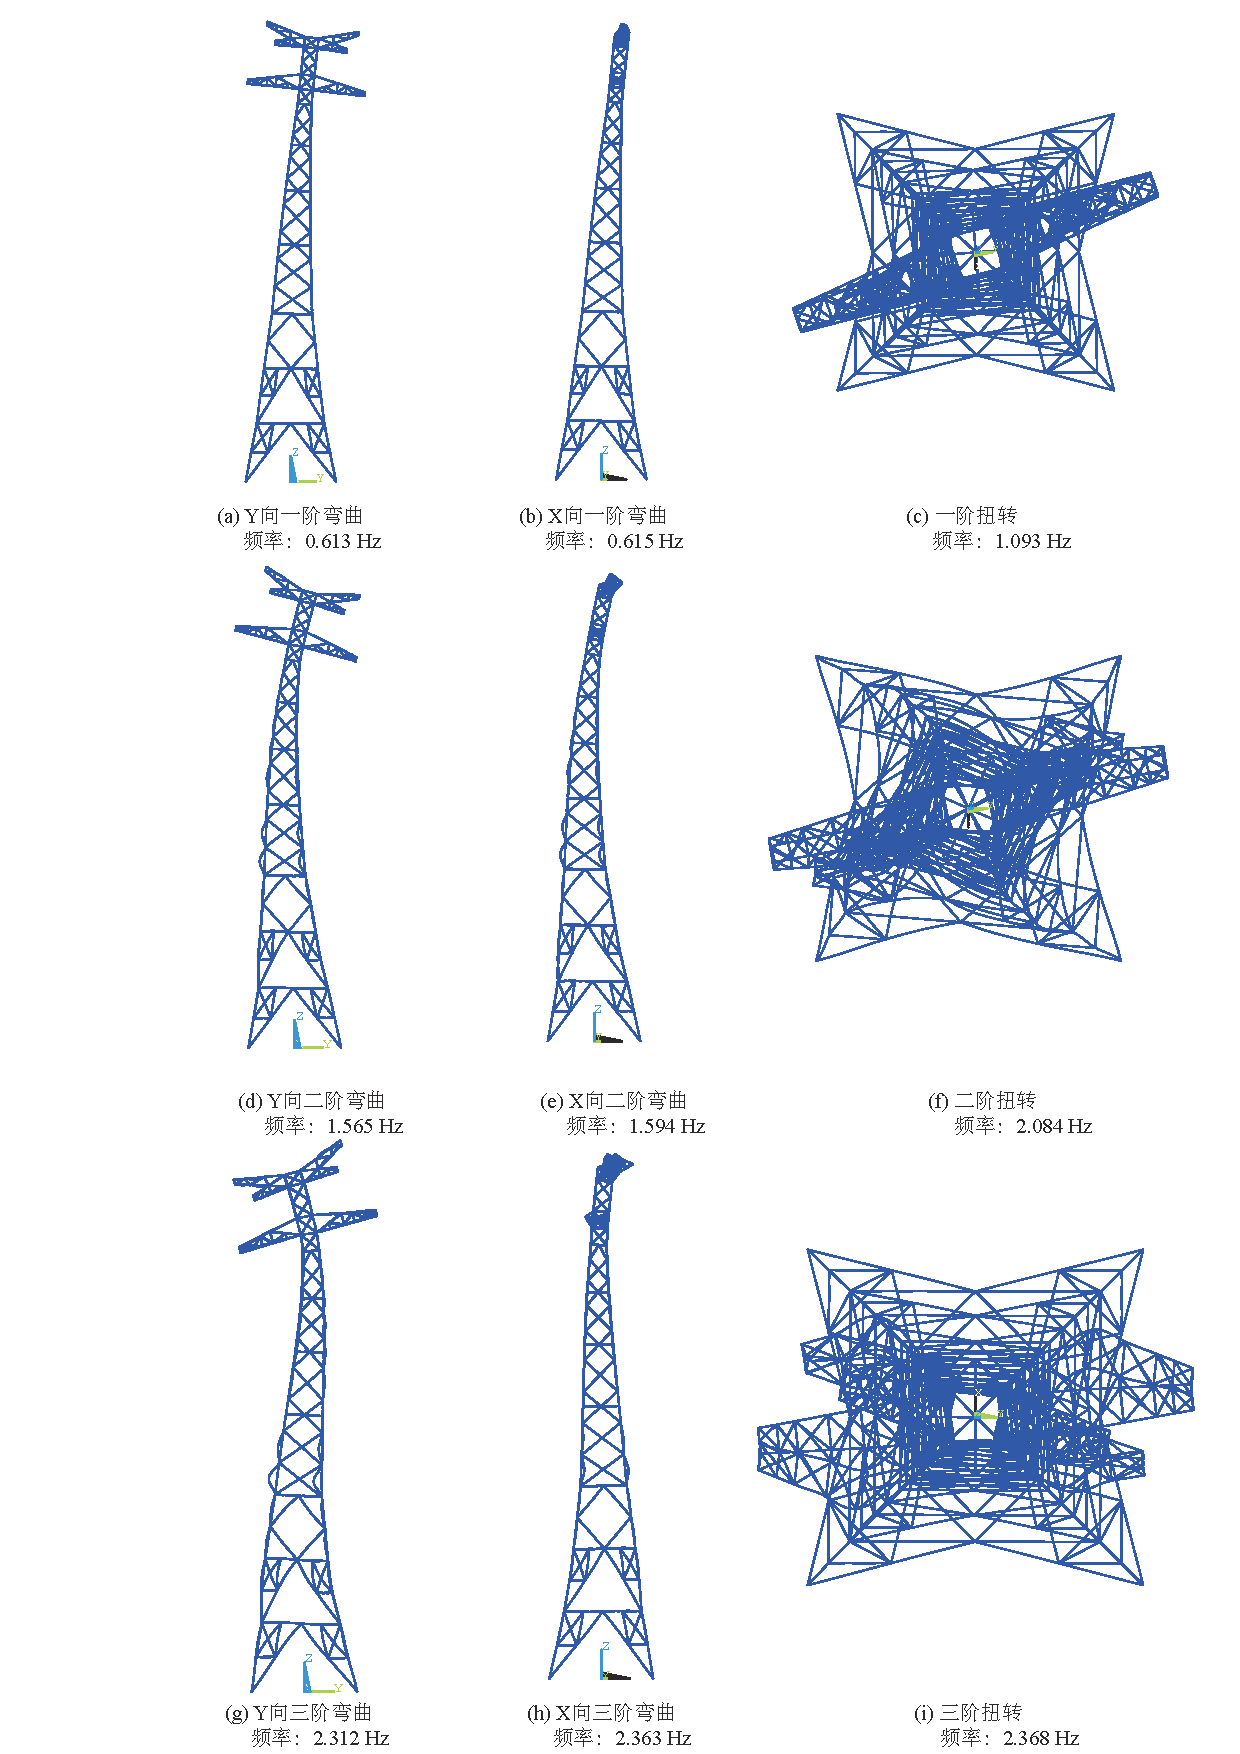
\includegraphics[width=0.9\textwidth]{modes.pdf}
	\caption{输电塔各阶振型图}
	\label{fig:modes}
\end{figure}

本章主要进行输电塔结构在龙卷风作用下的静态响应分析,即忽略龙卷风的平移效应,选定龙卷风核心相应于输电塔结构中心的位置,进行静力弹塑性分析。输电塔结构受到的主要荷载为:
\begin{enumerate}
	\item 重力荷载
	\item 输电塔受到的龙卷风涡旋风场的荷载
	\item 输电线传到输电塔的荷载
\end{enumerate}
其中忽略了龙卷风对输电线的荷载,主要是因为:
\begin{enumerate}
	\item 龙卷风路径宽度较小,F1-F2级龙卷风的路径宽度为\SI{60}{m}-\SI{150}{m}。
	\item 输电线受到的风荷载作用机制比较复杂。
\end{enumerate}

\section{输电塔龙卷风荷载计算的FSI方法}

\subsection{单向流固耦合方法介绍}
单向流固耦合分析(One-way Fluid Structure Interaction, FSI)以解耦的形式进行\cite{benra2011comparison}\cite{qian2008fsi}:
首先,将结构表面视为刚性的流场壁计算流场的分布;
然后将流场计算得到的刚性壁面压力施加到结构上以计算其响应。
单向流固耦合方法适用于结构在流场作用下变形较小(相比于流场的计算区域),即流场的边界改变较小,几乎不影响流场的分布情况。

\subsection{包含输电塔刚性模型的龙卷风风场}\label{sec:tornado-fsi}
输电塔结构可分为梁柱主体框架和支撑体系,将输电塔整体的刚性模型包含进风场时,发现划分的网格数量巨大,需要较长时间才能完成CFD计算。
故本文采用的方法如下:
首先在SolidWorks中用实体建立输电塔结构主体梁柱框架模型,忽略迎风效应(截面)较小的支撑等构件,然后从代表足尺龙卷风风场的圆柱体中利用布尔运算减去输电塔梁柱实体,生成包含输电塔刚性模型的计算流域。
支撑等构件受到的风荷载的计算方法在第\ref{sec:brace-load}节中介绍。

在该计算流域上设置第\ref{sec:full-tornado}足尺龙卷风风场的边界条件,并将输电塔刚性模型表面的边界条件设置为不可滑移壁面。
利用ICEM CFD软件进行网格划分,先采用Octree算法将计算流域初步划分为六面体和四面体混合的非结构化网格,再将生成的网格以Delaunay算法进行优化。
网格划分过程采用以下选项提高网格质量:控制输电塔表面网格划分的最大单元尺寸为\SI{0.4}{m};
同时在输电塔表面设置厚度为\SI{1.0}{m}的棱柱形单元膨胀层网格(Prism Layers);
并以输电塔中心建立半径为\SI{150}{m}的球状区域,在此区域内进行网格加密以尽可能精确离散结构表面。
计算流域底部和输电塔刚性模型表面的网格划分见图\ref{fig:mesh}所示。

考虑到龙卷风风场压强分布的梯度较大,故CFD计算采用PISO求解方法,压强离散采用PRESTO!格式\cite{fluent2015user}。

\begin{figure}[!htpb]
	\centering
	\includegraphics[width=\textwidth]{mesh.png}
	\caption{输电塔周围计算流域网格}
	\label{fig:mesh}
\end{figure}

设置输电塔结构表面的压强积分值为求解监测值,迭代过程中当残差和压强积分检测值趋于稳定时结束计算。
\SI{20}{m}高度处流场剖面速度矢量分布和结构表面风压云图分别见图\ref{fig:velocity}和图\ref{fig:pressure}所示。
后处理提取输电塔梁柱表面受到的风压,格式为风压点坐标及风压值,见表\ref{tab:pressure}所示。

\begin{figure}[!htpb]
	\centering
	\includegraphics[width=0.8\textwidth]{velo.jpg}
	\caption{\SI{20}{m}高度处风速矢量图}
	\label{fig:velocity}
\end{figure}

\begin{figure}[!htpb]
	\centering
	\includegraphics[width=0.5\textwidth]{pres.png}
	\caption{输电塔表面风压}
	\label{fig:pressure}
\end{figure}

\begin{table}[!htbp]
	\caption{输电塔表面CFD风压输出}
	\label{tab:pressure}
	\centering
	\begin{tabu} to 1.0\textwidth {X[c] X[c] X[c] X[1.5,c]}
		\toprule
		$X(\mathrm{m})$ & $Y(\mathrm{m})$ & $Z(\mathrm{m})$ & Pressure$(\mathrm{Pa})$ \\
		\midrule
		-94.756         & -95.510         & 0.000           & 1.906E+03               \\
		-45.910         & -94.756         & 0.000           & -1.664E+03              \\
		$\vdots$        & $\vdots$        & $\vdots$        & $\vdots$                \\
		-69.484         & -95.910         & 249.707         & 8.067E+02               \\
		\bottomrule
	\end{tabu}
\end{table}

\subsection{龙卷风风压转化为输电塔梁单元节点集中力}
在ANSYS Mechanical APDL中采用梁单元模拟输电塔结构,这就带来了CFD计算得到的龙卷风风压如何施加到梁单元上的问题。
设计如下算法以实现风压转化为梁单元节点集中力。
由于流场网格对刚性输电塔表面的离散,使得风压点的位置与实际的输电塔结构表面存在偏差。
因此需要设计算法实现如下功能:

\begin{figure}[!htbp]
	\centering
	\includegraphics{algo.pdf}
	\caption{CFD风压点$P$与梁单元$IJ$示意图}
	\label{fig:algo}
\end{figure}

\begin{itemize}
	\item 判别每个CFD风压点作用于哪个有限元梁单元。
	\item 将单个CFD风压点的风压(垂直于该风压点作用的梁单元的表面)分解到整体坐标系中。
	\item 将单个有限元梁单元所受所有CFD风压点的压力进行合成,并分配到该单元节点上。
\end{itemize}

任意CFD风压点$P$与某个梁单元$IJ$示意图见图\ref{fig:algo},图中点$P'$为风压点$P$在梁单元轴线$IJ$上的投影。
由于本文研究的输电塔为钢管塔,即梁$IJ$的表面为柱面,设其外径为$R_{IJ}$,则$PP'$即为风压作用于梁$IJ$的方向。
首先通过如下准则判断风压点$P$是否作用于梁单元$IJ$上:

\begin{itemize}
	\item $P'$是否在线$IJ$内部?
	\item $PP'$是否近似等于单元$IJ$外径?
\end{itemize}
当同时满足这两个条件时,认为风压点$P$作用于梁单元$IJ$上,数学表达见式\eqref{eqn:cri}。
\begin{gather}\label{eqn:cri}
	\bm{P'I}\cdot\bm{P'J} < 0  \nonumber \\
	|PP'-R_{IJ}| < \varepsilon
\end{gather}
式中点$P'$的坐标可由式\eqref{eqn:op}计算,
\begin{equation}\label{eqn:op}
	\bm{OP'}=\bm{OI} - \left( \frac{\bm{PI}\cdot\bm{IJ}}{|IJ|^2} \right)\bm{IJ}
\end{equation}
风压点$P$作用于梁单元$IJ$上的风压在整体坐标系下的分量为
\begin{equation}
	(p_X, p_Y, p_Z) = p\frac{\bm{PP'}}{|PP'|}
\end{equation}

根据上述判别法则,对每个CFD风压点与每根梁单元进行判别,可确定每根梁单元所受的所有CFD风压点及各自的风压分量。
下面介绍将单个有限元梁单元所受所有CFD风压点的压力进行合成,并分配到该单元节点上的方法。
\begin{enumerate}
	\item 计算单个有限元梁单元$IJ$受到的所有风压点处风压分量的平均$\bar{p_X},\bar{p_Y},\bar{p_Z}$;
	\item 将风压根据梁表面面积转化为合力$F_X=2\pi R_{IJ} |IJ| \bar{p_X}$,$Y,Z$方向类似;
	\item 将风压合力分量平分到梁单元$I$、$J$节点上。
\end{enumerate}
至此,完成了将CFD风压传递给有限元梁单元节点荷载的算法。
算法的Python程序见附录\ref{apen:load}。

\subsubsection{测试算例}
设计如图\ref{fig:example}所示的算例测试该算法的有效性。
悬臂钢管柱外径$R=\SI{1.0}{m}$,高度$H=\SI{9}{m}$,单侧受到径向压强,分布为$p_r(y)=p_0\frac{y}{H},p_0=\SI{100}{Pa}$。
据此编程生成风压点及相应的压强值,作为本文算法的输入,输出各节点施加的集中力见表\ref{tab:example-force}所示。
计算各节点集中力的合力见表\ref{tab:example-force},与理论合力$F_X = \int_{0}^{H}\int_{\pi/2}^{3\pi/2}p_r(y)\cos(\theta+\pi)R \mathrm{d} \theta \mathrm{d} y = p_0 RH=\SI{900}{N}$误差很小。

\begin{figure}[!htbp]
	\centering
	\includegraphics{example.pdf}
	\caption{测试算例示意图}
	\label{fig:example}
\end{figure}

\begin{table}[!htbp]
	\caption{测试算例输出节点集中力}
	\label{tab:example-force}
	\centering
	\begin{tabu} to 1.0\textwidth {X[c] X[2,c] X[2,c] X[2,c]}
		\toprule
		Node   & $F_X(\SI{}{N})$ & $F_Y(\SI{}{N})$ & $F_Z(\SI{}{N})$ \\
		\midrule
		1      & 5.527           & 0.000           & 0.000           \\
		2      & 22.526          & 0.000           & 0.000           \\
		3      & 44.996          & 0.000           & 0.000           \\
		4      & 66.994          & 0.000           & 0.001           \\
		5      & 88.994          & 0.000           & 0.001           \\
		6      & 110.991         & 0.000           & 0.000           \\
		7      & 132.990         & 0.000           & -0.002          \\
		8      & 154.990         & 0.000           & -0.001          \\
		9      & 176.987         & 0.000           & 0.002           \\
		10     & 93.992          & 0.000           & 0.002           \\
    \midrule
		$\sum$ & 898.987         & 0.000           & 0.003           \\
		\bottomrule
	\end{tabu}
\end{table}

\subsection{输电塔支撑构件的龙卷风荷载计算}\label{sec:brace-load}
利用APDL命令流从输电塔结构有限元模型中提取相应于支撑构件的梁单元节点编号及坐标。
并通过下述方法计算支撑构件梁单元所受龙卷风荷载的方法。

首先,支撑构件梁单元某节点受到的风荷载可由下式计算\cite{savory2001modelling}:
\begin{equation}
	\bm{F_w} = \frac{1}{2} \rho_a C_d A |U| \bm{U}
\end{equation}
式中,$\rho_a$为空气密度,$C_d$为体型系数,本位取为$1.0$,$A$为该节点迎风投影面积,$\bm{U}$为风场在该节点处的风速矢量。
编制fluent UDF(见附录\ref{apen:inter})程序提取任意支撑节点$P(x, y, z)$在第\ref{sec:tornado-fsi}节模拟风场中的速度,算法如下:

\begin{enumerate}
	\item
	      首先判断出点$P$所在的计算流域网格控制体(可通过点$P$与某控制体各表面形心连线的向量与控制体表面法向量的关系判断点 是否属于该控制体);
	\item
	      提取该控制体的中心$C$点坐标$(x_c, y_c, z_c)$和$C$处的流场速度分量和速度梯度分量(将速度和各方向速度分量梯度矢量记为$\bm{U_C}$和$\bm{G_{CX}}$、$\bm{G_{CY}}$、$\bm{G_{CZ}}$);
	\item
	      利用下式计算点$P$处$X$方向速度分量为
	      \begin{equation}
	      	U_{PX} = U_{CX} + (\bm{OP}-\bm{OC})\cdot \bm{G_{CX}}
	      \end{equation}
	      $Y$和$Z$方向速度分量可类似计算。
\end{enumerate}


\section{输电塔龙卷风荷载计算的规范方法}\label{sec:static-code}

\subsection{龙卷风风场处理}
输电塔在龙卷风风场中的水平投影示意图如图\ref{fig:tower-tornado-cs}所示。
\begin{figure}[!htpb]
	\centering
	\includegraphics[width=\textwidth]{tower_tornado_cs.pdf}
	\caption{输电塔在龙卷风风场中的水平投影示意图}
	\label{fig:tower-tornado-cs}
\end{figure}
输电塔直角坐标系$\{O: XYZ\}$的建立方法见第\ref{sec:tower-fea}节。
$abcd$为输电塔处于同一水平剖面的节点。
下文主要展示推导$d$节点处龙卷风风速的方法,其余节点类似。
龙卷风中心在坐标系$\{O: XYZ\}$中的位置用极坐标$(R, \theta)$表示。
输电塔节点$d$相应于龙卷风核心的极坐标为$(R_{fd}, \theta_{fd})$,$d$节点受到的龙卷风切向、径向风速分别为$V_{td}$、$V_{rd}$,以及图\ref{fig:tower-tornado-cs}未明确表示的竖向风速$V_{ad}$。

\subsubsection{输电塔节点相应于龙卷风中心位置的极坐标}\label{sec:d-polor}
假设$d$节点在输电塔坐标系$\{O: XYZ\}$中的坐标为$(x_d, y_d, z_d)$,下文将推导节点$d$相应于龙卷风中心的极坐标$(R_{fd}, \theta_{fd})$。

龙卷风中心$T(R, \theta)$在输电塔坐标系$\{O: XYZ\}$中的直角坐标为$(R\cos\theta, R\sin\theta)$,则节点$d$相应于龙卷风中心$T$的向量为:
\begin{equation}
	\vv{Td} = \vv{Od} - \vv{OT} = (x_d - R\cos\theta, y_d - R\sin\theta) = R_{fd}(\cos\theta_{fd}, \sin\theta_{fd})
\end{equation}
式中,
\begin{equation}
	\begin{split}
		R_{fd} & = \sqrt{(x_d-R\cos\theta)^2+(y_d-R\sin\theta)^2} \\
		\theta_{fd} & = \arctan \frac{y_d - R\sin\theta}{x_d - R\cos\theta}
	\end{split}
\end{equation}

\subsubsection{龙卷风风场在直角坐标系下的分量}\label{sec:cs}
第\ref{sec:tornado}节模拟的龙卷风风场是定义在极坐标系下的,而施加风荷载采用直角坐标系下的风速分量较为简单,因此需要将龙卷风风场从极坐标系转化为直角坐标系。

输电塔节点$d$受到的龙卷风径向风速$V_{rd}$与$X$轴正方向的夹角为$\theta_{fd}$(图\ref{fig:tower-tornado-cs}),切向风速$V_{td}$与$X$轴正方向的夹角为$(\theta_{fd}+\pi/2)$,进行速度的分解如下:
\begin{equation}
	\begin{split}
		V_{xd} & = V_{rd} \cos\theta_{fd} + V_{td} \cos(\theta_{fd}+\pi/2) \\
		& = V_{rd} \cos\theta_{fd} - V_{td} \sin(\theta_{fd}) \\
		V_{yd} & = V_{rd} \sin\theta_{fd} + V_{td} \sin(\theta_{fd}+\pi/2) \\
		& = V_{rd} \sin\theta_{fd} + V_{td} \cos(\theta_{fd}) \\   
		V_{zd} & = V_{ad}  
	\end{split}
\end{equation}

有了上述准备工作,就可以计算输电塔上任意节点受到的龙卷风风速在直角坐标系下的分量了。

\subsubsection{龙卷风风场中任意节点处风速分量}
输电塔节点$d$相应于龙卷风中心的实际位置为$(R_{fd}, \theta_{fd})$(见第\ref{sec:d-polor}节),此节点对应于缩尺龙卷风风场$V_r(r,z)$、$V_t(r,z)$和$V_a(r,z)$(见第\ref{sec:tornado}节)中的位置为$(R_{md}, Z_{md})$,且
\begin{equation}
	\begin{split}
		R_{md} & = R_{fd} / L_s \\
		Z_{md} & = z_{fd} / L_s
	\end{split}
\end{equation}

在缩尺龙卷风风场中,由位置$(R_{md}, Z_{md})$可提取缩尺龙卷风风场径向、切向和竖向风速分量分别为$V_{rmd}$、$V_{tmd}$和$V_{amd}$。根据缩尺龙卷风速度相似比$V_s$可将其转化为足尺龙卷风风场中的速度分量:

\begin{equation}
	\begin{split}
		V_{rd} &= V_{rmd} \times V_s \\
		V_{td} &= V_{tmd} \times V_s \\
		V_{ad} &= V_{amd} \times V_s
	\end{split}
\end{equation}

最后根据第\ref{sec:cs}节的方法即可将输电塔节点$d$受到的极坐标系下的足尺龙卷风风速分量转化为直角坐标系下的风速分量。


\subsection{输电塔结构龙卷风风荷载计算}
\subsubsection{ASCE输电塔荷载规范风荷载计算方法}
ASCE主编的输电塔荷载规范 Guidelines for electrical transmission line structural loading\cite{wong2009guidelines}中输电塔风荷载计算公式为:
\begin{equation}
	F = \gamma_{\mathrm{w}} Q K_{\mathrm{z}} K_{\mathrm{zt}} \left( V_{50}\right)^2 G C_{\mathrm{f}} A
\end{equation}
其中:
\begin{description}[leftmargin=!,labelwidth=2em]
	\item[$F$] 顺风向风荷载
	\item[$\gamma_{\mathrm{w}}$] 考虑平均重现期的风荷载调整系数。平均重现期为$50$年时,$\gamma_{\mathrm{w}}=1.0$;平均重现期为$100$年时,$\gamma_{\mathrm{w}}=1.15$
	\item[$V_{50}$] 平均重现期为$50$年规定的风速基准值(基本风速)
	\item[$K_{\mathrm{z}}$] 风速压力暴露系数
	\item[$K_{\mathrm{zt}}$] 地形系数
	\item[$Q$] 将风速转化为速度压的常数,$Q=1/2 \rho_a=\SI{0.613}{kg/m^3}$
	\item[$G$] 阵风系数
	\item[$C_{\mathrm{f}}$] 风压系数
	\item[$A$] 迎风面构件的投影面积
\end{description}
各量中文翻译参考刘刚的论文\cite{liu2010wind}。

下面介绍ASCE规范中输电塔结构所受风荷载的风压系数$C_{\mathrm{f}}$的计算方法。

风压系数是密实度系数(solidity ratio)$\Phi$的函数,定义为:
\begin{equation}
	\Phi = \frac{A_\mathrm{m}}{A_\mathrm{o}}
\end{equation}
其中:
\begin{description}[leftmargin=!,labelwidth=2em]
	\item[$A_\mathrm{m}$] 迎风面构件的投影面积
	\item[$A_\mathrm{o}$] 塔架的轮廓面积
\end{description}
风压系数与密实度系数$\Phi$的关系表见参见规范 Guidelines for electrical transmission line structural loading \cite{wong2009guidelines}中表 2-4和表2-5。

%图\ref{fig:force-coefficient}\cite{wong2009guidelines}

% \begin{figure}[!htbp]
% 	\centering
% 	\includegraphics[width=\textwidth]{force_coefficient.png}
% 	\caption{风压系数}\label{fig:force-coefficient}
% \end{figure}
% 方形截面的风压系数根据图\ref{fig:force-coefficient}中Table 2-4计算,圆形截面的风压系数根据Table 2-4的系数再乘上Table 2-5中的系数。

\subsubsection{中国架空输电线路设计规范风荷载计算方法}
中国《110~750kV架空输电线路设计规范》\cite{GB50545-2010}中杆塔风荷载的计算公式为:
\begin{equation}
	W_{\mathrm{s}} = W_{0} \cdot \mu_{\mathrm{z}} \cdot \mu_{\mathrm{s}} \cdot B_{2} \cdot A_{\mathrm{s}} \cdot \beta_{\mathrm{z}}
\end{equation}
\begin{equation}
	W_0 = V^2/1600
\end{equation}
式中:
\begin{description}[leftmargin=!,labelwidth=2em]
	\item[$W_{\mathrm{s}}$] 杆塔风荷载标准值(\SI{}{kN});
	\item[$W_{0}$] 基准风压标准值(\SI{}{kN/m^2});
	\item[$V$] 基准高度为\SI{10}{m}的风速(\SI{}{m/s});
	\item[$\mu_{\mathrm{z}}$] 风压高度变化系数
	\item[$\mu_{\mathrm{s}}$] 构件的体型系数,杆塔取$1.3(1+\eta)$,环形截面钢筋混凝土杆取$0.7$;
	\item[$B_{2}$] 杆塔构件覆冰风荷载增大系数,\SI{5}{mm}冰区取$1.1$,\SI{10}{mm}冰区取$1.2$,\SI{15}{mm}冰区取$1.6$,\SI{20}{mm}冰区取$1.8$,\SI{20}{mm}以上冰区取$2.0$~$2.5$;
	\item[$A_\mathrm{s}$] 迎风面构件的投影面积计算值(\SI{}{m^2});
	\item[$\eta$] 塔架背风面荷载降低系数,按表\ref{tab:eta}选用;
	\item[$\beta_\mathrm{z}$] 杆塔风荷载调整系数。
\end{description}

\begin{table}[!htbp]
	\caption{塔架背风面荷载降低系数$\eta$}
	\label{tab:eta}
	\centering
	\begin{tabu} to 1.0\textwidth {X[2,c] | X[c] X[c] X[c] X[c] X[c] X[c] }
		\toprule
		\diagbox{$b/a$}{$A_s/A$} & $\leq$ 0.1 & 0.2  & 0.3  & 0.4  & 0.5  & $>$ 0.6 \\
		\midrule
		$\leq$ 1                 & 1.0        & 0.85 & 0.66 & 0.50 & 0.33 & 0.15    \\
		2                        & 1.0        & 0.90 & 0.75 & 0.60 & 0.45 & 0.30    \\
		\bottomrule
	\end{tabu}
\end{table}

\subsubsection{中美规范计算输电塔龙卷风荷载参数取值}
美国输电塔荷载规范Guidelines for electrical transmission line structural loading\cite{wong2009guidelines}针对输电塔受到的龙卷风风荷载的建议为:考虑F2等级的龙卷风荷载,因为F2等级龙卷风发生的概率较高,且能够在经济投入允许的情况下加以设防;由于龙卷风风场速度为阵风风速,故风速压力暴露系数$K_\mathrm{z}$和阵风系数$G$取为$1.0$,即利用龙卷风风场的实际风速代入公式计算,不利用系数$K_\mathrm{z}$对其进行修正;由于龙卷风荷载是一种极端荷载情况,故考虑平均重现期的风荷载调整系数$\gamma_\mathrm{w}$取为$1.0$。

文献\cite{hamada2010finite}\cite{hamada2011behaviour}\cite{altalmas2014finite}等建议地形系数$K_\mathrm{zt}$取为$1.0$,因为龙卷风多发生在平坦开阔的平原。

参考美国输电塔荷载规范计算龙卷风荷载的参数取值建议,中国《110~750kV架空输电线路设计规范》的相关参数建议为:忽略覆冰荷载的影响,故杆塔构件覆冰风荷载增大系数取为$1.0$;忽略龙卷风的风振效应,将杆塔风荷载调整系数取为$1.0$。

\subsubsection{输电塔龙卷风荷载施加方法}
将输电塔分为多层,见图\ref{fig:tower-zone}所示,某具体层示意图见图\ref{fig:tower-zone-diagram}。
输电塔节点a,b,c和d上受到的龙卷风荷载的计算步骤如下:
\begin{figure}[!htbp]
	\centering
	\includegraphics[width=0.8\textwidth]{tower_zone.png}
	\caption{输电塔分层示意图}\label{fig:tower-zone}
\end{figure}

\begin{figure}[!htbp]
	\centering
	\includegraphics[width=0.4\textwidth]{tower_zone_diagram.png}
	\caption{输电塔典型层示意图}\label{fig:tower-zone-diagram}
\end{figure}

\begin{enumerate}
	\item 根据第\ref{sec:tornado}节计算输电塔节点a,b,c和d处龙卷风速度分量 $V_x$和$V_y$;
	\item 分别沿$X$和$Y$方向计算风速风量的均值$V_x'$和$V_y'$;
	\item 计算输电塔节点a,b,c和d处所在层龙卷风荷载,值得注意的是公式中各物理量采用SI单位制,即风速单位为\SI{}{m/s},风荷载单位为\SI{}{N}。
	      
	      根据美国ASCE规范,该层$X$和$Y$方向龙卷风荷载$F_{\mathrm{w}x}$和$F_{\mathrm{w}y}$为
	      \begin{equation}
	      	F_{\mathrm{w}x} = 0.613 (V_{x}')^2 C_{\mathrm{f}x} A_x
	      \end{equation}
	      \begin{equation}
	      	F_{\mathrm{w}y} = 0.613 (V_{y}')^2 C_{\mathrm{f}y} A_y
	      \end{equation}
	      其中,$A_x$和$A_y$分别为该层迎风面构件沿$X$和$Y$方向的投影面积。
	      风压系数由ASCE规范\cite{wong2009guidelines}中表2-4和表2-5计算。
	      
	      根据中国规范,该层$X$和$Y$方向龙卷风荷载$F_{\mathrm{w}x}$和$F_{\mathrm{w}y}$为
	      \begin{equation}
	      	F_{\mathrm{w}x} = 0.625 (V_{x}')^2 \mu_{\mathrm{s}x} A_x 
	      \end{equation}
	      \begin{equation}
	      	F_{\mathrm{w}y} = 0.625 (V_{y}')^2 \mu_{\mathrm{s}y} A_y 
	      \end{equation}
	      体型系数$\mu_\mathrm{s} = 1.3(1+\eta)$,$\eta$由表\ref{tab:eta}计算。
	      
	      可知中美规范计算龙卷风荷载的公式的主要区别如下:中国将风速转化为速度压的系数为$\SI{0.625}{kg/m^3}$,美国为$1/2\rho_a=\SI{0.613}{kg/m^3}$,中国规范稍微偏保守;二者的主要差别为体型系数(风压系数)的计算:对于圆形截面输电塔,$\Phi<0.025$的层,美国规范的风压系数为$C_\mathrm{f}=4.0\times0.67=2.68$,中国规范为$\mu_\mathrm{s}=1.3(1+\eta)=1.3 \times(1+1.0)=2.6$,相差不大,美国规范偏保守。
	      
	\item 迎风面和背风面上风荷载分配
	      
	      中国规范根据塔架背风面荷载降低系数$\eta$对某层输电塔所受风荷载进行分配,即迎风面节点在$X$和$Y$方向所受风荷载分量分别为 $1/(1+\eta) F_{\mathrm{w}x}$ 和 $1/(1+\eta) F_{\mathrm{w}y}$;背风面节点在$X$和$Y$方向所受风荷载分量分别为 $\eta/(1+\eta) F_{\mathrm{w}x}$ 和 $\eta/(1+\eta) F_{\mathrm{w}y}$;
	      
	\item 迎(背)风面节点间风荷载分配
	      
	      迎(背)风面上的节点根据各节点的投影面积进行迎(背)风面上风荷载的分配。
	      
	      
\end{enumerate}


\subsection{索的悬链线理论及输电线作用于塔的荷载}

\subsubsection{索的悬链线理论基本假设}
索由高强钢丝集束而成,相对抗弯刚度很小,其受力特点可以认为是完全柔性。
在自重和张力作用下分析其线形和力学参数时,基本假设如下:
\begin{itemize}
	\item
	      索是理想柔性,既不能受压也不能受弯;
	\item
	      索的材料符合胡克定律;
	\item
	      索的横截面积在外荷载作用下的变化量十分微小,可忽略不计。
\end{itemize}

为了确定重力作用下索的线形,以弦左端点为原点、竖直向上为Y轴正方向建立右手直角坐标系。
则索受到的重力沿Y轴负向。
假设单位长度索的质量恒定,且不随张力变化。

\begin{figure}[!htbp]
	\centering
	\includegraphics[width=0.6\textwidth]{catenary_diagram.pdf}
	\label{fig:catenary}
	\caption{索段计算示意图}
\end{figure}

\subsubsection{符号约定}
\begin{description}
	\item[$s$]
	从索左端点(坐标系原点)开始计算的索长度;
	\item[$\mu$]
	单位长度索的质量(假设是恒定的);
	\item[$T(s)$]
	索长度为$s$处的索张力(根据柔性索假设,张力沿索的切线方向);
	\item[$T_y(s)$]
	索长度为$s$处的索张力的$Y$向分量;
	\item[$T_x$]
	张力的$X$向分量(任取索段进行受力分析,由$X$向平衡方程可知$T_x$沿索长是均匀的);
	\item[$\theta(s)$]
	索切向量与$X$轴正向的夹角。
\end{description}

\subsubsection{自重作用下的单索线形求解}
索段竖向的平衡方程为\cite{bhattacharya2010time}:
\begin{gather}
	T_y(s) = g \int_{s^0}^{s} \mu \mathrm{d}s + T_y^0 \notag \\
	T_x \tan(\theta(s)) = g \mu \int_{s^0}^{s} \mathrm{d}s + T_y^0 \notag \\
	T_x \frac{\mathrm{d} y}{\mathrm{d} x} = g \mu \int_{s^0}^{s} \sqrt{1+\left(\frac{\mathrm{d} y}{\mathrm{d} x}\right)^2} \mathrm{d}x + T_y^0 \notag \\
	\frac{\mathrm{d}^2 y}{\mathrm{d} x^2} = \frac{g \mu}{T_x} \sqrt{1+\left(\frac{\mathrm{d} y}{\mathrm{d} x}\right)^2}
\end{gather}
此二阶微分方程的解析解为:
\begin{equation}
	y = \frac{T_x}{g \mu} \cosh \left( \frac{g \mu}{T_x} + c_1 \right)+c_2
\end{equation}
式中,$c_1$和$c_2$为由边界条件确定的积分常量。代入边界条件:$x=0,y=0;x=L,y=C$(见图\ref{fig:cat})。

\begin{figure}[!htpb]
	\centering
	\includegraphics[width=0.8\textwidth]{cat.pdf}
	\caption{单缆尺寸及边界条件示意图}
	\label{fig:cat}
\end{figure}

\begin{equation}
	\left \{
	\begin{aligned}
		  & \beta = \frac{g \mu L}{2 T_x}                                \\
		  & c_1 = \sinh^{-1}\left(\frac{\beta C / L}{\sinh \beta}\right) \\
		  & c_2 = -\frac{T_x}{g \mu} \cosh(c_1)                          
	\end{aligned}
	\right.
\end{equation}

悬链线索的形状长度$S$和无应力长度$S_0$分别为:
\begin{equation}
	S = \frac{T_x}{g\mu}\left[\sinh\left(\frac{g \mu L}{T_x}+c_1\right)+\sinh(c_1)\right]
\end{equation}

\begin{equation}
	\begin{split}
		S_0 &= S-\Delta S \\
		&= S - \frac{T_x}{EA g \mu }\left[ \frac{1}{2} g \mu L + \frac{1}{8} T_x \left( e^{2(c_1+2\beta)} - e^{-2(c_1-2\beta)} -e^{2c_1} + e^{-2c_1} \right) \right]
	\end{split}
\end{equation}

\subsubsection{输电线施加在输电塔的荷载求解}

跨越塔之间输电线跨度为$L=\SI{1770}{m}$,右侧支座比左侧支座高度相同,即$C=\SI{0}{}$,跨中矢高$f=\SI{132.4}{m}$,单位长度质量$\mu=\SI{3219}{kg/km}$。
索的弹性模量$E=\SI{108070}{MPa}$,截面积$A=\SI{729}{mm^2}$。
假设在外荷载作用下两支座的间距及高差保持不变。
主要任务是利用上述悬链线理论计算输电线对输电塔施加的荷载。

主要思路:输电线在自重和张力作用下,其线形为悬链线,故可采用悬链线经典公式来进行求解。
采用直接建模的方式,单缆采用LINK1单元模拟,单元水平长度为\SI{1}{m}。
分析时,首先假定水平力大小,根据悬链线方程求解节点坐标,由此建立节点和单元,并分析单缆在自重作用下的内力和线形。
如果求解获得的水平力与假定水平力之间的误差较大或者单缆变形较大,则返回重新计算,直至满足误差要求。计算框图如图\ref{fig:flow-chart}所示。

\begin{figure}[!htpb]
	\centering
	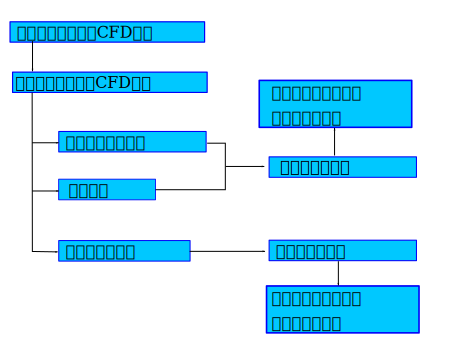
\includegraphics[width=0.6\textwidth]{flow_chart.pdf}
	\caption{单缆线形和力学参数计算框图}
	\label{fig:flow-chart}
\end{figure}

计算的APDL和MATLAB程序见附录\ref{apen:cat}。
单缆最大位移为\SI{12.7}{mm},相比于跨径$L=\SI{1770}{m}$该变形已足够小,认为已满足精度要求。

对于跨越塔和锚塔之间的输电线对跨越塔的荷载计算采用相同的方法,在此不一一列举。

跨越塔受到的两侧输电线传来的张力的示意图见图\ref{fig:line-force}所示。

\begin{figure}[!htbp]
	\centering
	\includegraphics[width=\textwidth]{line_force}
	\caption{跨越塔受到输电线的张力示意图}
	\label{fig:line-force}
\end{figure}

经过附录\ref{apen:cat}程序的计算,图\ref{fig:line-force}中各量为:
\begin{equation}
	\begin{split}
		T_{Lx} & = \SI{93.31}{kN},\quad \theta_L  = \ang{16.89} \\
		T_{Rx} & = \SI{21.33}{kN},\quad \theta_L  = \ang{36.70}
	\end{split}
\end{equation}


\section{FSI方法与规范方法的对比}\label{sec:static-results}

为了考虑最不利工况,将龙卷风核心距离输电塔中心的径向距离设置为龙卷风核心半径$R_T=r_{c,\mathrm{mat}}=\SI{120}{m}$,
$\theta_T$分别取\SI{0}{\degree}、\SI{45}{\degree}和\SI{90}{\degree}。
分别根据单向流固耦合方法(FSI方法)和规范方法计算并施加龙卷风荷载,进行输电塔结构的静态响应分析。
输电塔结构最大轴向压力和位移响应随袭击角$\theta_T$的变化见图\ref{fig:fx-vs-theta}和图\ref{fig:disp-vs-theta}所示。
代表性构件(见图\ref{fig:tower-zone}所示)的轴向力取得极值的工况见表\ref{tab:axial-force}所示。

\begin{figure}[!htbp]
	\centering
	\includegraphics[width=0.8\textwidth]{Fx_vs_theta.png}
	\caption{输电塔构件最大轴向压力随袭击角的变化}
	\label{fig:fx-vs-theta}
\end{figure}

\begin{figure}[!htbp]
	\centering
	\includegraphics[width=0.8\textwidth]{Disp_vs_theta.png}
	\caption{输电塔构件最大位移分量随袭击角的变化}
	\label{fig:disp-vs-theta}
\end{figure}

\begin{table}[!htbp]
	\caption{输电塔代表构件的轴向力}
	\label{tab:axial-force}
	\centering
	\begin{tabu} to 1.0\textwidth {X[c] X[c] X[2,c] X[c] X[2,c] X[c]}
		\toprule
		\multicolumn{2}{c}{构件} & \multicolumn{2}{c}{单向流固耦合} & \multicolumn{2}{c}{规范方法} \\
		编号 & 类型 & 轴向内力(\SI{}{kN}) & 角度(\SI{}{\degree}) & 轴向内力(\SI{}{kN}) & 角度(\SI{}{\degree}) \\
		\midrule
		C1	& 柱	& -6485	& 90 & 	-7803	& 90  \\
        C2	& 柱	& 7739	& 0	 &   8154	& 0  \\
        C3	& 柱	& -4958	& 90 &	-5024	& 90  \\
        C4	& 柱	& 5700	& 0	 &   5762	& 0  \\
        B1	& 梁	& 328	& 90 &	488	    & 90  \\
        B2	& 梁	& -274	& 0	 &  -316	& 0  \\
        B3	& 梁	& 87	& 0	 &   120	& 90  \\
        B4	& 梁	& -123	& 90 &	-130	& 90  \\
        Br1	& 支撑	& -27	& 45 &	-51	    & 45  \\
        Br2	& 支撑	& -42	& 45 &	-71	    & 45  \\
        Br3	& 支撑	& 318	& 90 &	588	    & 90  \\
        Br4	& 支撑	& -268	& 0	 &  -371	& 0  \\
		\bottomrule
	\end{tabu}
\end{table}

采用单向流固耦合和规范方法计算得到的输电塔结构响应整体上吻合较好,图\ref{fig:fx-vs-theta}和\ref{fig:disp-vs-theta}中按两种方法计算的结构轴向力和位移响应随袭击角$\theta_{\mathrm{T}}}$的变化趋势相似,且轴向力误差不超过$20\%$,位移响应误差不超过$30\%$,可以互相验证。
袭击角为\SI{45}{\degree}工况下结构在$X$和$Y$方向均发生变形,会出现整体的扭转变形。
表\ref{tab:axial-force}中所列构件中,梁柱等关键构件轴向力误差较小,支撑等次要构件轴向力响应误差较大,但误差不超过$50\%$。


\section{本章小结}

本章分别利用单向流固耦合方法和规范方法计算并施加龙卷风荷载到输电塔结构有限元模型上,并在0度,45度和90度袭击角工况下比较了两种方法计算得到的结构响应。

首先根据\SI{500}{kV}南京三江口大跨越工程中跨越塔建立有限元模型,并进行模态分析提取结构固有频率,与文献进行对比以验证结构有限元模型的正确性。

然后在忽略龙卷风平移运动的影响下,选定龙卷风核心相应于输电塔结构中心的位置,进行静力弹塑性分析。
输电塔受到的龙卷风荷载分别通过单向流固耦合方法和规范中风荷载公式计算。

单向流固耦合方法直接在足尺龙卷风风场中建立结构主体梁柱框架的刚性模型,通过CFD计算得到刚性模型表面受到的龙卷风风压,并编程将风压转化为输电塔梁单元模型的节点集中力;
对于支撑等迎风效应(截面尺寸)较小的构件,直接提取风场中相应于支撑构件节点处的风速,并利用阻力系数将风速转化为节点荷载。
将这两部分荷载均施加到结构有限元模型上,进行静力弹塑性分析,进而提取结构响应。

规范方法先对足尺龙卷风数值风场进行处理,转化成切向、径向风速在不同高度处随径向距离的分布;
并推导公式计算输电塔任意节点受到龙卷风在整体直角坐标系下风速分量;
然后简要比较了美国Guidelines for electrical transmission line structural loading规范和中国《110 ~ 750kV 架空输电线路设计规范》中风荷载计算公式,并将输电塔结构分成多层,分层施加龙卷风荷载。

输电塔还受到输电线传来的荷载,本章利用索的悬链线理论进行计算。

最后考虑最不利工况,将龙卷风核心与输电塔中心的距离设置为龙卷风核心半径$R_T=r_{c,max}=\SI{120}{m}$,袭击角分别取为$\SI{0}{\degree}$、$\SI{45}{\degree}$和$\SI{90}{\degree}$。
分别利用单向流固耦合方法和规范方法计算龙卷风荷载,分析比较结构的最大轴向力和位移响应。
发现采用单向流固耦合和规范方法计算得到的输电塔结构响应整体上吻合较好,按两种方法计算的结构轴向力和位移响应随袭击角的变化趋势相似,且最大轴向力误差不超过$20\%$,最大位移响应误差不超过$30\%$,可以互相验证。
\SI{45}{\degree}工况下结构在$X$和$Y$方向均发生变形,会出现整体的扭转变形。
两种方法计算的代表性构件的轴力,梁柱等关键构件轴力误差较小,支撑等次要构件轴向力响应误差较大,但误差不超过$50\%$。

%%% Local Variables:
%%% mode: latex
%%% TeX-PDF-mode: t
%%% TeX-engine: xetex
%%% TeX-master: "../main"
%%% End:

\graphicspath{{figures/dynamic/}}

\chapter{考虑龙卷风平移的动态响应分析}

\section{动态龙卷风模型}

\section{动态龙卷风风速及荷载时程}

\section{输电塔结构动态时程分析}



\chapter{结论与展望}

\section{全文总结}

本文利用CFD数值模拟技术,分析了龙卷风作用下输电塔结构的准静态和动态响应。
选取\SI{500}{kV}南京三江口长江大跨越工程中跨越塔为研究对象,分别以单向流固耦合方法和规范方法计算结构受到的龙卷风荷载,分析比较龙卷风袭击角为\SI{0}{\degree}、\SI{45}{\degree}时的准静态响应;
并考虑龙卷风的平移运动,进行输电塔结构在龙卷风动态荷载作用下的时程分析。
本文的研究成果可为输电塔结构的抗龙卷风设计提供一定的参考。
本文的主要研究内容和结论可概括为以下几点:

1)简要介绍了龙卷风这种破坏力巨大的极端气象灾害,包括其风场特性及造成的经济损失。
综述了当前龙卷风研究方法的现状,包括现场实测、试验模拟和数值分析。
根据目前国内输电塔结构抗龙卷风研究的现状,本文说明了研究课题的意义和主要的研究思路。

2)依据文献中龙卷风试验模拟为基础建立了CFD缩尺龙卷风风场,发现缩尺风场的切向风速的分布与Rankine涡模型及试验测得的风速分布吻合较好,呈现的风速分布特征为:
切向速度在涡旋中心处较小,随着离涡旋中心的距离增大而增大,在核心半径处达到最大,而后随着远离涡旋中心的距离增大而逐渐减小;
且沿径向分布时,在核心半径内,切向速度变化较快,而远离核心半径时,变化逐渐缓和。
然后将缩尺龙卷风数值风场与1998年发生在Spencer地区的实测龙卷风风场进行对比,通过引入长度相似比和速度相似比的概念将缩尺缩尺风场模型改造成足尺龙卷风风场模型。
发现当长度相似比取为$4000$、速度相似比取为$60$时,龙卷风足尺数值风场与Spencer龙卷风实测风场吻合较好。

3)探讨了龙卷风袭击角分别为$\SI{0}{\degree}$、$\SI{45}{\degree}$和$\SI{90}{\degree}$工况时输电塔结构的静态响应。
分别利用单向流固耦合方法和规范方法计算龙卷风荷载,分析比较结构的最大轴向力和位移响应。
发现采用单向流固耦合和规范方法计算得到的输电塔结构响应整体上吻合较好,按两种方法计算的结构轴向力和位移响应随龙卷风袭击角的变化趋势相似,且最大轴向力误差不超过$20\%$,最大位移响应误差不超过$30\%$,可以互相验证两种龙卷风荷载计算方法。
\SI{45}{\degree}工况下结构在$X$和$Y$方向均发生变形,会出现整体的扭转变形。
单向流固耦合方法和规范方法计算得到的输电塔结构在龙卷风作用下的代表性构件的轴力,发现梁柱等关键构件轴力误差较小,支撑等次要构件轴向力响应误差不超过$50\%$。

4)考虑龙卷风的平移运动,  选取龙卷风移动路径平行和垂直于输电线的两种典型工况,在任意时间步利用规范方法计算并施加龙卷风动态荷载,进行动力时程分析,并分析龙卷风动态荷载和结构典型响应的时程。
结果表明,平行工况下龙卷风荷载总和时程在输电线方向的分量出现持续时间约为\SI{10}{s}的波形(荷载先逐渐增大,后逐渐衰减),且荷载峰值较大,呈现出一定的冲击效应。
垂直工况下龙卷风荷载总和时程在垂直输电线方向的分量出现类似的特点。
且在两种工况下,输电塔塔顶节点位移时程与龙卷风荷载总和时程变化趋势相似。


\section{研究展望}

龙卷风是一种小尺度气旋,破坏力极强,近年来成为风工程领域里研究的热点。
龙卷风的数值模拟方法克服其他方法,如现场实测和试验模拟等的一些不足之处,具有方便、快速、经济和高效率等优势。
本文利用CFD数值方法模拟了输电塔结构受到的龙卷风荷载,并改变龙卷风核心相对于输电塔结构的位置,进行龙卷风作用下的准静态分析和动力时程分析。
本文得到一些建设性的结论,但仍然存在许多不完善的地方。
今后可考虑从以下几个方面进行完善。

1)实测的龙卷风存在多涡形态,且受地面粗糙度,研究者认为实测的龙卷风涡流比约为$2.0$,本文模拟的风场涡流比为$0.28$,故本文模拟的数值龙卷风与实际情况存在差距。
今后可考虑通过引入更为精细的数值模拟方法(如大涡模拟等),以模拟出更为符合实际的龙卷风风场。

2)本文忽略了输电线受到的龙卷风作用,这主要是考虑到龙卷风尺度相比输电线长度较小,且输电线受到的风荷载作用机理较为复杂。
本文还忽略了输电线与塔的耦合作用,这种耦合作用在动力时程分析中会产生较大的阻尼,但考虑这一作用会引起结构有限元分析的较强非线性。
今后的研究可考虑输电线受到的龙卷风荷载和输电线与塔的耦合作用。

3)本文中龙卷风作用下输电塔结构的准静态分析考虑了结构材料非线性和几何非线性,但考虑龙卷风移动效应的动力时程分析中假定结构处于弹性状态。
这主要是由于动力时程分析计算量较大,笔者不具有足够的计算资源实施动力弹塑性分析。
今后的研究可考虑动力时程分析中结构的材料非线性和几何非线性,进而进行倒塌性分析。

4)真实的龙卷风风场中风致飞射物对结构的打击作用不容忽视,也是造成结构破坏的一个重要因素。
本文在此未考虑风致飞射物的影响。
今后的研究中可根据龙卷风强度,对不同形状、不同质量的飞射物的运动轨迹进行模拟,以确定风致飞射物对建筑结构的影响。


%%% Local Variables:
%%% mode: latex
%%% TeX-PDF-mode: t
%%% TeX-engine: xetex
%%% TeX-master: "../main"
%%% End:


\thesisbib{seuthesix}

\acknowledgement

转眼间已到了毕业季,也是我在南京生活的第七年了。
七年的青春先后在东南大学九龙湖校区和四牌楼校区度过,所学所思,伴我一生。

感谢导师吕令毅教授,引导我寻找课题、比较研究方法,谆谆教诲「做人做事做学问」的理念。
吕老师治学严谨求实,生活简单健康,为人质朴淡泊名利,亦追求卓越,不断进取。
若无吕老师的悉心启迪与引领,难有我论文顺利完成。
在此,万分感谢恩师。

感谢江苏省电力设计院张晋绪师兄提供南京三江口大跨越输电塔工程的设计参数,
并指导了输电塔结构的相关知识。

良好的课题组氛围令我的论文工作充满了思维碰撞的乐趣。
感谢已走上工作岗位的师兄(姐)刘道勇、王宁、宋拓、汤卓、唐飞燕、彭英海、张弛的辛勤指导,帮助良多。
师兄徐康,师弟张良辰、胡婉亭、吴熙、刘远之,同门许逸文、王美珍朝夕相处,探讨课题,获益匪浅。
文昌十二舍601,陈凯、刘震、朱冬平自本科便相识,相伴近六年,时而鼓励,催我奋进,时而倾听,解我烦忧,已成一生挚友。

论文准备和撰写期间使用了许多优秀的开源软件,感谢其开发者和社区维护者,他们的工作令论文的书写多了优雅和享受,包括Emacs编辑器,{\LaTeX} 排版系统和Python编程语言。

最后感谢我平凡伟大的父母和亲爱的弟弟,他们的支持与奉献,给了我无穷的勇气和毅力完成学业。

%%% Local Variables:
%%% mode: latex
%%% TeX-PDF-mode: t
%%% TeX-engine: xetex
%%% TeX-master: "../main"
%%% End:


\appendix
\chapter{龙卷风数值模拟速度入口处边界条件的UDF程序}
\begin{minted}{c}
#include "udf.h"

#define H 0.4
#define R 0.4
#define UREF 0.34    /* reference velocity */
#define ZREF 0.025    /* reference height */
#define S 0.28    /* swirl ratio */

/* profile for radial velocity */
DEFINE_PROFILE(V_r, t, i)
{
    real x[ND_ND], z;
    face_t f;

    begin_f_loop(f, t)
    {
        F_CENTROID(x, f, t);
        z = x[2];
        F_PROFILE(f, t, i) = -UREF*pow(z/ZREF,1.0/7.0);
    }
    end_f_loop(f, t)
}

/* profile for tangential velocity */
DEFINE_PROFILE(V_t, t, i)
{
    real x[ND_ND], z;
    face_t f;

    begin_f_loop(f, t)
    {
        F_CENTROID(x, f, t);
        z = x[2];
        F_PROFILE(f, t, i) = 2.0*S*UREF*pow(z/ZREF,1.0/7.0);
    }
    end_f_loop(f, t)
}

\end{minted}

\chapter{风压转化为梁节点集中力的Python程序}\label{apen:load}

\section{main.py}
\begin{minted}{python}
import numpy as np

import reader as rd
import crossSele as cs
import pNormIJ as pIJ

loadOut = 'load.csv'
epsilon = 0.01

# Initiate Matrix elePres to hold pressure on
# elemnt (eleNum, presX, presY, presZ)
elePres = np.zeros((rd.elemCount, 5))
elePres[:, 0] = range(1,rd.elemCount+1)

print("Start to map the CFD Pressure Points to Elements...")

for p in range(rd.presCount):
    # p iterate all the cfd pressure points
    XP = rd.cfdPresM[p, 0:3]    # Coordinates of point p+1
    pres = rd.cfdPresM[p, 3]    # pressure of point p+1
    
    # decide cfd pressure point (p+1) belongs to which element
    for e in range(rd.elemCount):
        # e interate all elements, e refers element (e+1)
        (dist, normVec, flag) = pIJ.pNormIJ(XP, cs.XIE(e+1), cs.XJE(e+1),\
            distEpsilon=cs.RoE(e+1)*(1+epsilon))   
        # compute the distance from point (p+1) to element (e+1)
        if flag:
            # cfd pressure point (p+1) belongs to element (e+1)
            elePres[e, 1:4] = elePres[e, 1:4] + pres*normVec
            elePres[e, 4] = elePres[e, 4] + 1
            print("CFD Pressure Point ({X:9.3f},{Y:9.3f},{Z:9.3f}) \
               belongs to Element {eleNum:6d}"\
               .format(X=XP[0], Y=XP[1], Z=XP[2], eleNum=e+1))
            break

print("CFD Pressure Points mapping ratio:{:6.3%}."\
  .format(sum(elePres[:,4])/rd.presCount))

print("Starting convert the CFD Pressure to Elemeng nodal force...")
# Transfer the element pressures to element node force
# Init nodeForce matrix to hold force on nodes (nodeNum, Fx, Fy, Fz)
nodeForce = np.zeros((rd.nodeCount, 4))
nodeForce[:, 0] = range(1,rd.nodeCount+1)

for e in range(rd.elemCount):
    # (e+1) interate all elements
    if elePres[e, 4] == 0:
        presMean = np.zeros((3,))
    else:
        presMean = elePres[e, 1:4] / elePres[e, 4]

    forceTotal = presMean * cs.AoE(e+1)
    nodeI = int(rd.eleM[e, 1])
    nodeJ = int(rd.eleM[e, 2])
    nodeForce[nodeI-1, 1:4] = nodeForce[nodeI-1, 1:4] + forceTotal/2
    nodeForce[nodeJ-1, 1:4] = nodeForce[nodeJ-1, 1:4] + forceTotal/2
    print("Element {eleNum:6d} nodal force \
                   F=({Fx:9.3f} N, {Fy:9.3f} N, {Fz:9.3f} N)"\
      .format(eleNum=e+1, Fx=forceTotal[0]/2, \
              Fy=forceTotal[1]/2, Fz=forceTotal[2]/2))


print("Sum FX is {:6.3f} N.".format(sum(nodeForce[:, 1])))
print("Sum FY is {:6.3f} N.".format(sum(nodeForce[:, 2])))
print("Sum FZ is {:6.3f} N.".format(sum(nodeForce[:, 3])))


with open(loadOut, 'w') as f:
    for n in range(rd.nodeCount):
        f.write('{NODE:6d}, {Fx:9.3f}, {Fy:9.3f}, {Fz:9.3f}\n'\
        .format(NODE=n+1, Fx=nodeForce[n, 1], Fy=nodeForce[n, 2],\
                Fz=nodeForce[n, 3]))

f.close()

\end{minted}

\section{reader.py}
\begin{minted}{python}
import numpy as np

inputDir = "Input/"
caseDir = "theta-0/"
# Read CFD Pressure Data (x[m], y[m], z[m], pres[Pa])
cfdPresFile = inputDir + caseDir + "cfd_pressure.csv"
cfdPresM = np.genfromtxt(cfdPresFile, delimiter=',', skip_header=17)
cfdPresM[:,3] = 1.0*cfdPresM[:,3]    # into the surface pressure +

# Read CFD velocity Data
# (nodeNum, x[m], y[m], z[m], pres[Pa], u[m/s], v[m/s], w[m/s])
cfdVeloFile = inputDir + caseDir + "cfd_velocity2.out"
cfdVeloM = np.genfromtxt(cfdVeloFile, delimiter=',')

# Remove the zero lines
cfdV = cfdVeloM[~np.all(cfdVeloM == 0.0, axis = 1)]
cfdV = cfdV[:, [0,5,6,7]]

# Read Node List File (nodeNum, nodeX[m], nodeY[m], nodeZ[m])
nodeFile = inputDir+"node_list.txt"
nodeM = np.genfromtxt(nodeFile, delimiter=',')

# Read Element List File (eleNum, eleI, eleJ, eleSecn)
eleFile = inputDir+"ele_list.txt"
eleM = np.genfromtxt(eleFile, delimiter=',')

# Read Section List File (secNum, Ro[m])
secFile = inputDir+"sec_list.txt"
secM = np.genfromtxt(secFile, delimiter=',')

presCount = np.size(cfdPresM, 0)    # total num. of cfd pressure points
nodeCount = np.size(nodeM, 0)    # total num. of nodes
elemCount = np.size(eleM, 0)    # total num. of elements
secCount = np.size(secM, 0)    # total num. of sections
veloCount = np.size(cfdV, 0)

\end{minted}

\section{pNormIJ.py}
\begin{minted}{python}
import numpy as np

def pNormIJ(CoordP=(0.0, 0.0, 0.0), CoordI=(1.0, 0.0, 0.0), \
                    CoordJ=(0.0, 1.0, 0.0), distEpsilon=1.0):
    """ Return the distance of point P to line IJ and the norm vector PP'
        where P' is the projection of P to IJ.

    Keyword arguments:
    CoordP -- the coordinates of point P, default (0.0, 0.0, 0.0)
    CoordI -- the coordinates of point I, default (0.0, 1.0, 0.0)
    CoordJ -- the coordinates of point J, default (0.0, 0.0, 1.0)
    distEpsilon -- distance criterion

    Return:
    dist -- distance from point P to line IJ
    normVec -- norm vector of PP'
    """
    CoordP = np.array(CoordP)
    CoordI = np.array(CoordI)
    CoordJ = np.array(CoordJ)
    CoordPPrime = np.zeros((3,))
    flag = False

    normIJ = np.linalg.norm(CoordI - CoordJ)
    CoordPPrime = CoordI + np.dot(CoordI-CoordP,\
        CoordI-CoordJ)/(normIJ**2)*(CoordJ-CoordI)
    dist = np.linalg.norm(CoordP-CoordPPrime)
    normVec = (CoordPPrime-CoordP)/dist

    if (np.dot(CoordPPrime-CoordI, CoordPPrime-CoordJ) < 0 and\
        dist < distEpsilon):
        flag = True

    return (dist, normVec, flag)
\end{minted}

\section{crossSele.py}  
\begin{minted}{python}
import numpy as np

import reader as rd

def XIE(eleNum=1):
    """ Get the coordinates of I node of Element eleNum.

    Keyword argument:
    eleNum -- element number
    """
    eINum = int(rd.eleM[eleNum-1][1])
    return rd.nodeM[eINum-1][1:]


def XJE(eleNum=1):
    """ Get the coordinates of J node of Element eleNum.

    Keyword argument:
    eleNum -- element number
    """
    eJNum = int(rd.eleM[eleNum-1][2])
    return rd.nodeM[eJNum-1][1:]


def RoE(eleNum=1):
    """ Get the Ro of section of Element eleNum.

    Keyword argument:
    eleNum -- element number
    """
    secNum = int(rd.eleM[eleNum-1][3])
    return rd.secM[secNum-1][1]

def AoE(eleNum=1):
    """ Get the surface area of Element eleNum.

    Keyword argument:
    eleNum -- element number    
    """
    length = np.linalg.norm(XIE(eleNum)-XJE(eleNum))
    return 2*np.pi*RoE(eleNum)*length

\end{minted}

%%% Local Variables:
%%% mode: latex
%%% TeX-master: "../main"
%%% End:

\chapter{CFD风场任意位置处风速的UDF插值程序}\label{apen:inter}
\begin{minted}{c}
#include "udf.h"

#define MAXPOINTS 5000
#define NSCALARS (1+ND_ND)

real coords[MAXPOINTS][ND_ND+1];
real values[MAXPOINTS][NSCALARS+ND_ND+1];

int total_count;
int total_points_found = 0;

FILE *input;
FILE *output;

int is_point_in_cell(cell_t c, Thread *t, real *x);

DEFINE_ON_DEMAND(interpolate)
{
    Domain *d = Get_Domain(1);
    Thread *t;
    cell_t c;

    real NV_VEC(x), NV_VEC(dx), NV_VEC(grady), NV_VEC(centroid);
    real y0, y;

    int point, i, n;
    int reader_flag;

    /* Read the Points data to array coords */
    input = fopen("node_list_0.txt", "r");

    for(i=0; i<MAXPOINTS; i++)
    {
        reader_flag = fscanf(input, "%f, %f, %f, %f\n",\
            &coords[i][0], &coords[i][1], &coords[i][2], &coords[i][3]);

        if (reader_flag!=4)
            break;

        total_count = i;
    }
    fclose(input);


    /* Initialize values */
    for(i=0; i<MAXPOINTS; i++)
    {
        for(n=0; n<NSCALARS+ND_ND+1; n++)
        {
            values[i][n] = 0.0;
        }
    }
    
    /* Interpolation starts ... */
    for(point=0; point<total_count; point++)
    {
        /* Get coords of point to vec x */
        for(i=0; i<ND_ND; i++)
            x[i] = coords[point][i+1];

        /* Find the cell of point */
        thread_loop_c(t, d)
        {
            begin_c_loop(c, t)
            {
                if (is_point_in_cell(c, t, x))
                {
                    C_CENTROID(centroid, c, t);
                    total_points_found++;
                    Message("The cell including point (%f,%f,%f) has\
                        centroid of (%f,%f,%f).\n",\
                        x[0],x[1],x[2],centroid[0],centroid[1],centroid[2]);

                    /* Store the coords */
                    values[point][0] = coords[point][0];
                    for(i=0; i<ND_ND; i++)
                    {
                        values[point][i+1] = x[i];
                    }

                    y0 = 0.0;
                    NV_VV(dx, =, x, -, centroid);
            
                    for(n=0; n<NSCALARS; n++)
                    {
                        switch (n)
                        {
                            case 0:
                                NV_V(grady, =, C_P_G(c,t));
                                y0 = C_P(c,t);
                                break;
                            case 1:
                                NV_V(grady, =, C_U_G(c,t));
                                y0 = C_U(c,t);
                                break;
                            case 2:
                                NV_V(grady, =, C_V_G(c,t));
                                y0 = C_V(c,t);
                                break;
                            case 3:
                                NV_V(grady, =, C_W_G(c,t));
                                y0 = C_W(c,t);
                                break;
                            default:
                                break;
                        }

                        y = y0 + NV_DOT(grady, dx);
                        values[point][ND_ND+n+1] = y;
                    }
                    break;
                }
            }
            end_c_loop(c, t)
        }
    }

    output = fopen("output.out","a");
    if (!output)
    {
        Message("\n\nERROR: Could not open interpolation output file.\n");
        return;
    }
    for(point=0; point<total_points_found; point++)
    {
        for(i=0; i<NSCALARS+ND_ND+1; i++)
        {
            fprintf(output, "%12.5f ", values[point][i]);
        }
        fprintf(output,"\n");
    }
    fprintf(output,"\n");
    fclose(output);

}


int is_point_in_cell(cell_t c, Thread *t, real *x)
{
    int i;
    face_t f;
    Thread *tf;
    real A[ND_ND], n[ND_ND], v[ND_ND], z[ND_ND];
    real face_centroid[ND_ND], cell_centroid[ND_ND];
    real Amag;

    /* Center of cell */
    C_CENTROID(cell_centroid, c, t);

    /* Loop over all faces of cell */
    c_face_loop(c, t, i)
    {
        /* Face i of cell */
        f = C_FACE(c, t, i);
        tf = C_FACE_THREAD(c, t, i);

        /* Face normal */
        F_AREA(A, f, tf);

        /* Normalize A to reduce truncation error */
        Amag = NV_MAG(A);
        NV_VS(n, =, A, /, Amag);

        /* Centroid on face i */
        F_CENTROID(face_centroid, f, tf);

        /* Vector from face centroid to point x */
        NV_VV(v, =, x, -, face_centroid);

        /* Vector from cell centroid to face centroid */
        NV_VV(z, =, face_centroid, -, cell_centroid);

        /* Perform test to make sure face normal points outwards */
        if (NV_DOT(n, z) < 0.0)
            NV_S(n, *=, -1.0);

        /* If n.v > 0, then point is beyond "plane" that defines 
           the face and it annot be inside the cell */
        if (NV_DOT(n, v) > 0.0)
            return 0;
    }
    
    /* Otherwise it must be in the cell */
    return 1;
}

\end{minted}

%%% Local Variables:
%%% mode: latex
%%% TeX-master: "interpolationUDF"
%%% End:

\documentclass[border=10pt]{standalone}
\usepackage{tikz}
\usetikzlibrary{arrows.meta}
\usepackage{structuralanalysis}

\begin{document}
\begin{tikzpicture}
  \point{O}{0}{0};
  \point{A}{3.7cm*3}{-1.6031cm*3};
  \draw[help lines,-Stealth] (O) -- (2,0) node[right] {$x$};
  \draw[help lines,-Stealth] (O) -- (0,1) node[left] {$y$};
  \draw[blue,scale=3] plot[blue] file {cat_diagram.csv};
  \foreach \x/\y in {0.25/-0.18063,0.5/-0.34998,0.75/-0.50828,1/-0.65573,1.25/-0.79255,1.5/-0.91892,1.75/-1.035,2.0/-1.141,2.25/-1.237,2.5/-1.3232,2.75/-1.3996,3/-1.4664,3.25/-1.5237,3.5/-1.5716}{
    \draw[scale=3,-Stealth] (\x,\y) ++(0,-0.02) -- ++(0,-0.15);
  };
  \draw[scale=3] (1.75,-1.035) ++(0,-0.2) node[below] {$q_y$};
  \support{1}{O};
  \hinge{1}{O};
  \draw[scale=3,red,-Stealth] (3.7,-1.6031) -- ++($0.5*(1,-0.1426)$) node[below right] {$T$};
  \draw[scale=3,red,dashed,-Stealth] (3.7,-1.6031) -- ++($0.5*(0,-0.1426)$) node[below] {$T_y$};
  \draw[scale=3,red,dashed,-Stealth] (3.7,-1.6031) -- ++($0.5*(1,0)$) node[right] {$T_x$};
  \draw[scale=3,help lines] (0,-1.8) -- (0,-2);
  \draw[scale=3,help lines] (3.7,-1.8) -- (3.7,-2);
  \draw[scale=3,help lines,Stealth-Stealth] (0,-1.9) -- (3.7,-1.9) node[above,pos=0.5] {$L$};
  \draw[scale=3,help lines] (4.5,0) -- (4.7,0);
  \draw[scale=3,help lines] (4.5,-1.6031) -- (4.7,-1.6031);
  \draw[scale=3,help lines,Stealth-Stealth] (4.6,0) -- (4.6,-1.6031) node[above,pos=0.5,rotate=90] {$C$};
  
\end{tikzpicture}
\end{document}

\resume{作者攻读硕士学位期间的研究成果}

 王勇(1991—),男,汉族,河南人,2014年毕业于东南大学土木工程专业,获工学学士学位。
 2014年免试攻读本校土木工程专业结构工程方向学术硕士学位。
 在校期间共学习课程13门,总计29学分,其中学位课程18学分,成绩良好。

\begin{flushleft}
{\bfseries \large 发表的论文}\\ \relax
[1] 王勇, 吕令毅. 龙卷风作用下输电塔结构的单向流固耦合分析[J]. 特种结构, 2017, 34(2): 13-19.
\\ \relax
[2] 王勇, 吕令毅. 龙卷风风场中块状飞射物飞行特性的CFD模拟[C]. 2016年东南大学校庆研究生学术报告会论文集
\\
 
\end{flushleft}
\end{document}

%%% Local Variables:
%%% mode: latex
%%% TeX-PDF-mode: t
%%% TeX-engine: xetex
%%% TeX-master: t
%%% End:
